\documentclass[12pt, letterpaper]{article}

% --- PACKAGES ---
\usepackage[margin=1in]{geometry}
\usepackage{setspace}
\setstretch{1.15}
\usepackage{times}
\usepackage[utf8]{inputenc}
\usepackage[T1]{fontenc}
\usepackage{xcolor}
\usepackage{cite}
\usepackage{amsmath,amssymb,amsfonts,amsthm}
\usepackage{algorithm}
\usepackage{algorithmic}
\usepackage{graphicx}
\usepackage{textcomp}
\usepackage{tikz}
\usetikzlibrary{shapes, arrows, positioning, calc, shadows, fit, backgrounds}
\usepackage{booktabs}
\usepackage{microtype}
\usepackage{url}
\usepackage{listings}
\usepackage{tabularx}
\usepackage[font=small,labelfont=bf]{caption}
\captionsetup[table]{skip=10pt}
\usepackage{hyperref}

% --- FIX: Load tcolorbox ONCE with the 'most' option ---
\usepackage[most]{tcolorbox}

% --- DEFINITIONS FOR GUARDS ---
\newcommand{\pred}[1]{\texttt{#1}}

\newtcolorbox{guardbox}[2][]{%
    colback=gray!5!white,
    colframe=gray!50!black,
    colbacktitle=gray!20!white,
    coltitle=black,
    fonttitle=\bfseries,
    title={#2},
    arc=2pt, boxrule=0.5pt,
    left=6pt, right=6pt, top=6pt, bottom=6pt,
    % --- ADDS BREATHING ROOM TO THE HEADING ---
    toptitle=4pt, bottomtitle=4pt,
    before skip=1em, after skip=1em,
    #1
}

% --- JSON LANGUAGE DEFINITION ---
\colorlet{punct}{red!60!black}
\definecolor{background}{HTML}{EEEEEE}
\definecolor{delim}{RGB}{20,105,176}
\colorlet{numb}{magenta!60!black}

\lstdefinelanguage{json}{
    basicstyle=\normalfont\ttfamily\footnotesize,
    numbers=left,
    numberstyle=\scriptsize,
    stepnumber=1,
    numbersep=8pt,
    showstringspaces=false,
    breaklines=true,
    frame=lines,
    backgroundcolor=\color{background},
    literate=
     *{0}{{{\color{numb}0}}}{1}
      {1}{{{\color{numb}1}}}{1}
      {2}{{{\color{numb}2}}}{1}
      {3}{{{\color{numb}3}}}{1}
      {4}{{{\color{numb}4}}}{1}
      {5}{{{\color{numb}5}}}{1}
      {6}{{{\color{numb}6}}}{1}
      {7}{{{\color{numb}7}}}{1}
      {8}{{{\color{numb}8}}}{1}
      {9}{{{\color{numb}9}}}{1}
      {:}{{{\color{punct}{:}}}}{1}
      {,}{{{\color{punct}{,}}}}{1}
      {\{}{{{\color{delim}{\{}}}}{1}
      {\}}{{{\color{delim}{\}}}}}{1}
      {[}{{{\color{delim}{[}}}}{1}
      {]}{{{\color{delim}{]}}}}{1},
}

% --- CODE LISTING STYLE ---
\lstset{
    basicstyle=\ttfamily\small,
    breaklines=true,
    frame=single,
    numbers=left,
    numberstyle=\tiny,
    xleftmargin=2em,
    framexleftmargin=1.5em
}

% --- THEOREMS ---
\newtheorem{definition}{Definition}
\newtheorem{proposition}{Proposition}
\newtheorem{lemma}{Lemma}
\newtheorem{corollary}{Corollary}
\newtheorem{theorem}{Theorem}
\newtheorem{remark}{Remark}
\newtheorem{assumption}{Assumption}
% --- FIX: This was missing and caused your error ---
\newtheorem{principle}{Principle}

% --- METADATA ---
\newcommand{\projectTitle}{Managing the Stochastic: Foundations of Learning in Neuro-Symbolic Systems for Software Engineering}
\newcommand{\studentName}{Matthew Thompson}
\newcommand{\submissionDate}{\today}


\begin{document}

% --- TITLE PAGE ---
\begin{titlepage}
    \centering
    \vspace*{1.5in}

    {\Huge \bfseries \projectTitle \par}

    \vspace{1.5in}

    {\Large \textbf{Matthew Thompson} \par}
    \vspace{0.1in}
    {\small ORCID: \href{https://orcid.org/0009-0007-0846-0369}{0009-0007-0846-0369} \par}
    \vspace{0.2in}
    {\large \textit{Independent Researcher} \par}

    \vspace{1.0in}

    {\large \submissionDate \par}

    \vfill

    % Optional: Add a note about the preprint status
    {\footnotesize \textit{Preprint submitted to arXiv.}}

    \vspace{0.3in}
    {\footnotesize \textcopyright\ 2025 Matthew Thompson. This work is licensed under a \href{https://creativecommons.org/licenses/by/4.0/}{Creative Commons Attribution 4.0 International License (CC BY 4.0)}. Code available under \href{https://github.com/thompsonson/atomicguard}{MIT License}.}
\end{titlepage}

% --- ABSTRACT ---

\begin{abstract}

Current approaches to AI coding agents appear to blur the lines between the Large Language Model (LLM) and the agent itself, asking the LLM to make decisions best left to deterministic processes. This leads to systems prone to stochastic failures such as gaming unit tests or hallucinating syntax. Drawing on established software engineering practices that provide deterministic frameworks for managing unpredictable processes, this paper proposes setting the control boundary such that the LLM is treated as a component of the environment environment---preserving its creative stochasticity---rather than the decision-making agent.

A \textbf{Dual-State Architecture} is formalized, separating workflow state (deterministic control flow) from environment state (stochastic generation). \textbf{Atomic Action Pairs} couple generation with verification as indivisible transactions, where \textbf{Guard Functions} act as sensing actions that project probabilistic outputs onto observable workflow state.

The framework is validated on three code generation tasks across 13 LLMs (1.3B--15B parameters). For qualified instruction-following models, task success rates improved by up to 66 percentage points at 1.2--2.1$\times$ baseline computational cost. The results suggest that architectural constraints can substitute for parameter scale in achieving reliable code generation.
\end{abstract}


\vspace{0.5cm}
\noindent \textbf{Keywords:} Neuro-symbolic AI, LLM Agents, Runtime Verification, Code Generation, Iterative Refinement, Software Engineering

\newpage

% --- TABLE OF CONTENTS ---
\tableofcontents
\newpage

% --- BODY OF TEXT ---

\section{Introduction}

\subsection{Motivation: A Formal Building Block for Software Engineering}

Modern software engineering has evolved sophisticated practices for managing complexity and uncertainty: CFEngine for infrastructure convergence, XP for iterative development, CI/CD for continuous validation, and Domain-Driven Design for semantic boundaries. These practices share a common thread—they provide deterministic frameworks for managing inherently unpredictable processes.

Large Language Models present a parallel challenge: substantial capability with stochastic behavior. While "Attention is All You Need" launched the transformer revolution, experience suggests that \textit{Attention is Not All You Need} for Software Engineering—robust systems also require the scaffolding of verification, convergence, and bounded autonomy. Just as CFEngine treats infrastructure as eventually consistent rather than immediately correct, LLM outputs are treated in this framework as eventually valid through iterative refinement.

This work does not propose a revolutionary new algorithm, but rather a formalization of these emerging architectural patterns. The contribution is a theoretical grounding of these heuristics—providing the vocabulary, convergence guarantees, and formal reasoning framework required to transform ad-hoc "guardrails" into rigorous engineering disciplines.

Specifically, this work formalizes the separation of deterministic control flow from stochastic content generation. Through \textbf{Atomic Action Pairs} (inseparable generation-verification units) and a \textbf{Dual-State Solution Space} (workflow state versus environment state), the framework enables LLMs to operate within traditional software engineering bounds. Each verification failure provides feedback that refines subsequent generation attempts, achieving reliability through iteration rather than perfection.

Additionally, the architecture provides a potential approach to the Credit Assignment Problem inherent in LLM training. By enforcing immediate verification the framework naturally generates immediate reward signals attributed to specific generation attempts, rather than the sparse rewards typical of end-to-end generation. These verified traces can support both online reinforcement learning and offline supervised fine-tuning (e.g., via LoRA). Over time, this could theoretically reduce retry rates from the observed 2.1× toward 1.0× as models internalize domain-specific constraints.

Importantly, this architectural approach enables reliable systems using smaller, locally-deployed models (< 15B parameters) rather than requiring API access to frontier models. By substituting architectural rigor for parameter scale, organizations can maintain control over their software development pipeline while achieving high reliability.

\begin{tcolorbox}[colback=gray!10, colframe=gray!60, title=Practitioner's Note]
If you have built production LLM systems, this formalization likely describes patterns you are already using. This paper's goal is not to prescribe new practices, but to provide the theoretical substrate that explains \textit{why} these patterns work and \textit{when} they provide guarantees.
\end{tcolorbox}


\subsection{Theoretical Context and Prior Art}

The control dynamics of this framework draw from convergence patterns first encountered in configuration management, where CFEngine was leading the way in applied research \cite{burgess1995site, burgess1998computer} and subsequently formalized as Promise Theory \cite{burgess2005autonomy, burgess2014promise}. In production systems, CFEngine demonstrated that reliability emerges not from commanding distributed components but from continuous convergence toward desired states—autonomous agents make promises rather than receive commands. This practical insight, later abstracted by Burgess into Promise Theory, provides the theoretical lens for managing stochastic systems: treat unreliable components as "promisers" and architect convergence operators to guide them toward validity.

Applied to LLMs, this convergence paradigm operates within the classical agent-environment boundary defined by Sutton \& Barto \cite{sutton2018reinforcement}, where the agent comprises only components modifiable by the control policy. Since the LLM's weights cannot be modified during inference, it resides in the environment, with the agent function—per Russell \& Norvig's formalization \cite{russell2020artificial}—mapping percepts (generation outputs) to actions (verification decisions).

Against this theoretical foundation, prior approaches to LLM control generally fall into two categories:

\begin{description}
    \item[External Control Architectures (Symbolic \& Hybrid):] Frameworks such as HTN planning \cite{erol1994htn} and LLM-Modulo \cite{kambhampati2024llms} maintain deterministic control outside the model. While logically sound, they rely on explicit causal models (preconditions/effects) which are notoriously difficult to extract from the latent space of black-box LLMs.

    \item[Internal Control Architectures (LLM-Centric):] Conversely, techniques like Chain-of-Thought \cite{wei2022chain} and ReAct \cite{yao2022react} locate the control loop inside the stochastic generation window. While flexible, these methods suffer from probabilistic control flow, where the agent's decision-making process is subject to the same hallucination modes as its content generation.
\end{description}

This framework synthesizes these perspectives by utilizing external symbolic guards to enforce the internal convergence of generative promises.


\subsection{Framework Overview}

Building on goal-based agent frameworks \cite{shen2014goalbasedagents}, this work introduces a mechanism to externalize reasoning. The definition of an action is extended to utilize guard functions—not merely as gates, but as active postcondition validators that project the LLM's internal generation process onto a verifiable external state.

These sensing actions enable a dual-state architecture that provides:

\begin{itemize}
    \item \textbf{Observable Workflow Reasoning:} Unlike opaque internal monologues (e.g., Chain-of-Thought), reasoning is captured in explicit state transitions, converting probabilistic generation into deterministic logical steps.
    \item \textbf{Bounded Indeterminacy:} The system guarantees termination and cost control through deterministic validation predicates and finite retry budgets.
    \item \textbf{Atomic Composition:} Generation and verification are treated as a single transactional unit—an "Atomic Action Pair"—ensuring that invalid content never pollutes the workflow state.
\end{itemize}

% --- FIGURE 1 (Final) ---
\begin{figure}[htbp]
    \centering
    \resizebox{\columnwidth}{!}{
    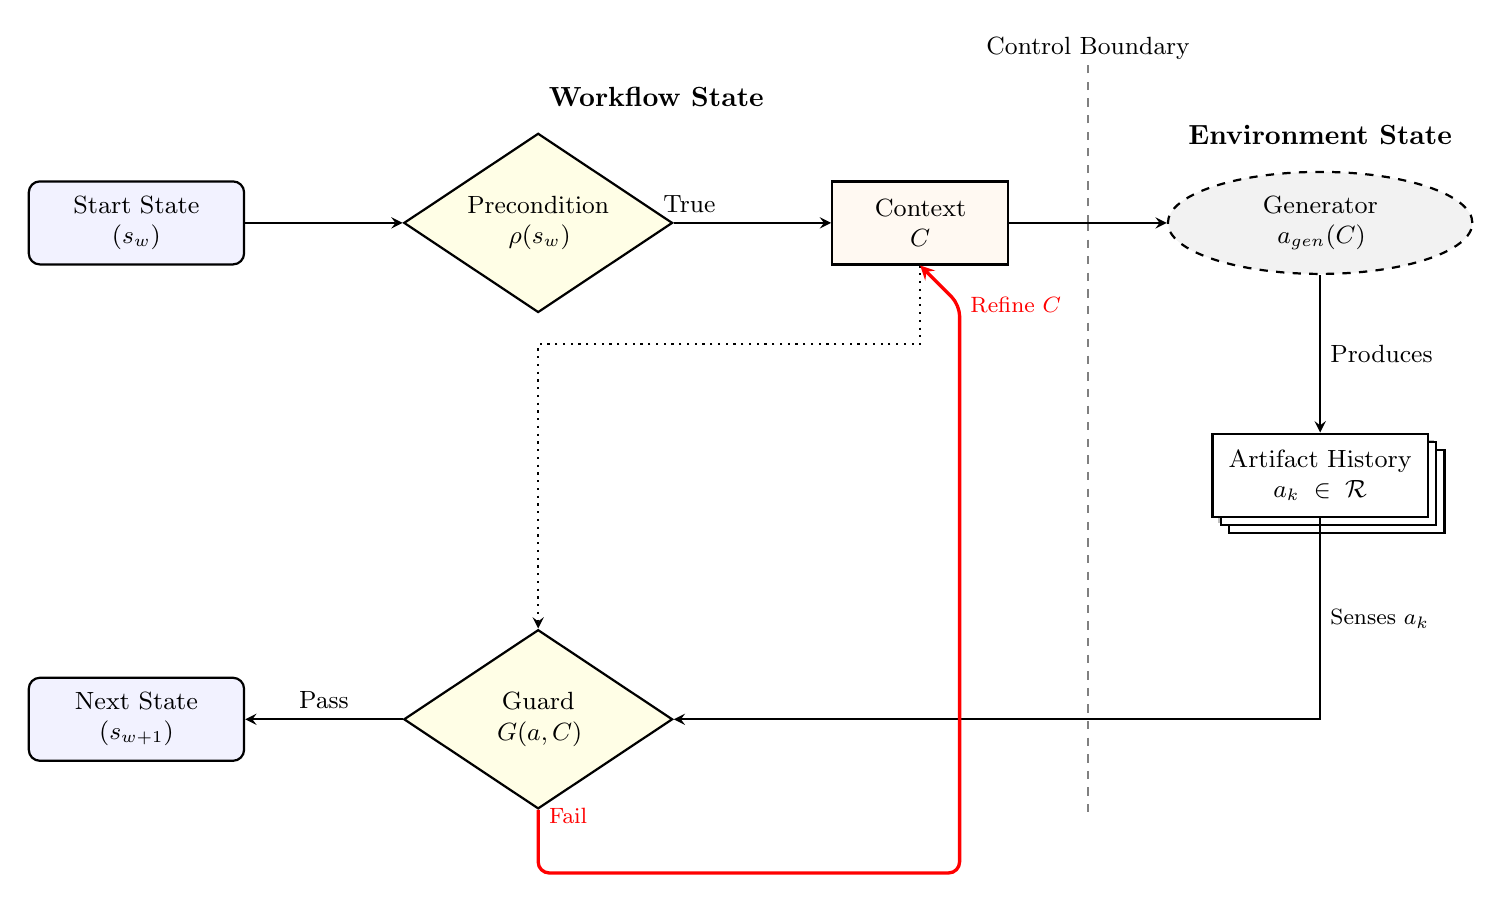
\begin{tikzpicture}[
        node distance=1.5cm and 2.0cm,
        auto,
        >=stealth,
        thick,
        font=\small,
        block/.style={rectangle, draw, fill=blue!5, text width=2.5cm, align=center, rounded corners, minimum height=3em},
        cloud/.style={ellipse, draw, fill=gray!10, text width=2.5cm, align=center, minimum height=3em, dashed},
        stack/.style={rectangle, draw, fill=white, text width=2.5cm, align=center, minimum height=3em, drop shadow={opacity=0.5}, double copy shadow={shadow xshift=3pt, shadow yshift=-3pt}},
        decision/.style={diamond, draw, fill=yellow!10, text width=1.8cm, align=center, aspect=1.5},
        context/.style={rectangle, draw, fill=orange!5, text width=2.0cm, align=center, minimum height=3em}
    ]

    % --- Observable World (Left: Agent) ---
    \node (start) [block] {Start State\\($s_w$)};
    \node (precond) [decision, right=of start] {Precondition\\$\rho(s_w)$};
    \node (ctx) [context, right=of precond] {Context\\$C$};

    % --- Opaque World (Right: Environment) ---
    \node (gen) [cloud, right=of ctx] {Generator\\$a_{gen}(C)$};
    \node (artifact) [stack, below=of gen, yshift=-0.5cm] {Artifact History\\$a_k \in \mathcal{R}$};

    % --- Boundary Line ---
    \draw[dashed, gray] ($(ctx.east)!0.5!(gen.west)$) coordinate (mid) -- +(0,-7.5) node[above, pos=-0.26, black] {Control Boundary};
    \draw[dashed, gray] (mid) -- +(0,2);

    % --- Forward Paths ---
    \draw[->] (start) -- (precond);
    \draw[->] (precond) -- node[above, pos=0.1] {True} (ctx);
    \draw[->] (ctx) -- (gen);
    \draw[->] (gen) -- node[right] {Produces} (artifact);

    % --- SENSING PATH (Artifact -> Guard) ---
    \node (guard) [decision, below=of precond, yshift=-2.5cm] {Guard\\$G(a, C)$};
    \draw[->] (artifact.south) |- node[near start, right, font=\footnotesize] {Senses $a_k$} (guard.east);

    % --- CONTEXT INPUT TO GUARD ---
    % Drawing a line from Context to Guard to show G(a, C) dependency
    \draw[->, dotted] (ctx.south) -- ++(0,-1.0) -| (guard.north);

    % --- Logic Paths ---
    \node (success) [block, left=of guard] {Next State\\($s_{w+1}$)};
    \draw[->] (guard) -- node[above] {Pass} (success);

    % --- RED FAILURE LOOP ---
    \draw[->, red, very thick, rounded corners]
        (guard.south) -- node[right, font=\footnotesize, pos=0.1] {Fail} ++(0,-0.8)
        -| ($(ctx.south) + (0.5, -0.5)$)
        -- node[right, font=\footnotesize, pos=0.0] {Refine $C$} (ctx.south);

    % Labels
    \node[above=0.2cm of gen, font=\bfseries] {Environment State};
    \node[above=0.2cm of precond, xshift=1.5cm, font=\bfseries] {Workflow State};

    \end{tikzpicture}
    }
    \caption{The Atomic Action Pair. The architecture enforces a strict separation between the Observable Workflow (left) and the Opaque Environment (right). The red loop illustrates the refinement transition: unlike standard backtracking, the workflow state $s_w$ remains invariant while guard feedback $\phi$ updates the generative context $C$. The dotted line indicates that the Guard conditions validation on both the artifact and the context.}
    \label{fig:atomic_pair}
\end{figure}


\section{Definitions}

To rigorously formalize the relationship between deterministic workflows and stochastic generators, foundational concepts in agency are distinguished from the specific architectural interpretations employed in this framework.

\subsection{Foundational Definitions}
\begin{description}
    \item[Promise Theory (Burgess, 2015)] A model of voluntary cooperation where autonomous agents issue promises regarding intended behavior rather than guarantees. Interactions are defined by the consumer's responsibility to verify promise fulfillment, replacing command-and-control assumptions.

    \item[Agent (Russell \& Norvig, 1995)] A function $f: \mathcal{P}^* \to \mathcal{A}$ mapping a complete percept history to actions. A rational agent selects actions that maximize an expected performance measure given its percept sequence and built-in knowledge.

    \item[Control Boundary (Sutton \& Barto, 1998)] The boundary defining the agent comprises only those components that can be arbitrarily modified by the control policy. Components outside this boundary constitute the environment.

    \item[Bounded Rationality (Simon, 1955)] Rational agents operating under computational constraints do not optimize for the global maximum; instead, they satisfice, selecting the first solution that meets the aspiration level (validity criteria) within the available search budget.

    \item[Weak Agency (Wooldridge \& Jennings, 1995)] A software system exhibiting autonomy, reactivity, and pro-activeness, without implying consciousness or mental states.
\end{description}

\subsection{Architectural Definitions}

\begin{description}
    \item[Control Boundary (Generative Application)] This framework applies Sutton \& Barto's definition to the resource-dependent nature of Large Language Models (LLMs). The agent boundary is defined by modifiability relative to the time horizon:
    \begin{itemize}
        \item \textit{Intra-Episode:} The agent controls context composition ($C$) and state transitions ($S_{workflow}$).
        \item \textit{Inter-Episode:} With sufficient compute, the agent may control adapter parameters (e.g., LoRA) or distilled weights.
        \item \textit{Base Model:} The pre-trained weights remain in the environment, providing a stochastic generation oracle that functions as the fixed generative component.
    \end{itemize}

    \item[Goal-Based Agent (Deterministic Controller)] A rational decision function $f: \mathcal{P}^* \to \mathcal{A}$ that treats stochastic generations as \textit{percepts} rather than actions. The agent observes the opaque output of the LLM (environment) and executes deterministic state transitions (actions) based on verification results. This ensures that while the \textit{content} is stochastic, the \textit{control flow} remains strictly deterministic.

    \item[Neuro-Symbolic Agentic System] A software architecture integrating neural generation with symbolic verification. The LLM (as a component of the environment) issues generation promises; deterministic guard functions verify promise fulfillment within an atomic transaction, ensuring that invalid states are never committed to the persistent workflow history.

    \item[Dual-State Architecture] An implementation pattern that separates the system state space $\mathcal{S}$ into two distinct spaces:
    \begin{itemize}
        \item $\mathcal{S}_{workflow}$ \textit{(Control State):} A deterministic, finite state machine tracking goal progress and guard satisfaction.
        \item $\mathcal{S}_{env}$ \textit{(Information State):} An append-only versioned repository of generation history, artifacts, and guard feedback, enabling in-context learning without polluting the control flow.
    \end{itemize}
\end{description}


% --- Section 2: Formal Framework ---
\section{Formal Framework}

\subsection{Dual State Space}
\begin{definition}[State Space Decomposition]
The system state space $\mathcal{S}$ is decomposed into an observable workflow space and an opaque environment space:
\begin{equation}
\mathcal{S} = \mathcal{S}_{\text{workflow}} \times \mathcal{S}_{\text{env}}
\end{equation}
\begin{itemize}
    \item \textbf{Workflow State ($\mathcal{S}_{\text{workflow}}$):} Defined as the set of all truth assignments to the guard functions:
    \begin{equation}
    \mathcal{S}_{\text{workflow}} = \{ \sigma \mid \sigma : \mathcal{G} \to \{\bot, \top\} \}
    \end{equation}
    where $\mathcal{G} = \{g_1, ..., g_n\}$ is the set of unique guard identifiers.

    \item \textbf{Environment State ($\mathcal{S}_{\text{env}}$):} Defined as the Cartesian product of the artifact space and context space:
    \begin{equation}
        \mathcal{S}_{\text{env}} = \mathcal{A} \times \mathcal{C}
    \end{equation}
    A specific environment state is denoted as a tuple $s_{\text{env}} = \langle a, C \rangle$, where $a \in \mathcal{A}$ is the current artifact (mutable result) and $C \in \mathcal{C}$ is the cumulative context (immutable history).
\end{itemize}
\end{definition}

\begin{remark}[Information Abstraction]
The workflow state acts as a finite abstraction of execution progress. While the guard function returns detailed feedback $\phi \in \Sigma^*$ (e.g., compiler logs), this information is projected into the opaque \textit{Context} ($\mathcal{C}$). Only the binary satisfaction signal $v \in \{\bot, \top\}$ is retained in $\mathcal{S}_{\text{workflow}}$, preserving the finiteness of the planning space.
\end{remark}

\subsection{Artifacts, Context, and Provenance}

To ensure auditability and enable effective backtracking, the environment is formalized not as a mutable store, but as an append-only versioned repository.

\begin{definition}[Artifact Space \& Versioning]
Let $\mathcal{A}$ be the set of all possible concrete outputs. A Versioned Repository $\mathcal{R}$ is defined as a Directed Acyclic Graph (DAG) where nodes represent artifact versions $a_v$ and edges represent derivation steps.
\[ \mathcal{R} = \{ (a_0, \dots, a_k) \mid a_i \in \mathcal{A} \} \]
Every generative action creates a new node in $\mathcal{R}$ rather than overwriting the previous state. This strictly preserves the failure history (``rejected branches'') for future learning.
\end{definition}

\begin{definition}[Hierarchical Context Composition]
The context $\mathcal{C}$ conditioning the generator and available to the guard is the composition of three distinct scopes:
\begin{equation}
    C_{total} = \langle \mathcal{E}, C_{local}, H_{feedback} \rangle
\end{equation}
\begin{itemize}
    \item \textbf{Ambient Environment ($\mathcal{E} = \langle \mathcal{R}, \Omega \rangle$):}
    Contains the \textbf{Versioned Repository $\mathcal{R}$} (providing read-only access to all finalized ancestor and cousin artifacts) and \textbf{Global Constraints $\Omega$}.

    \item \textbf{Local Context ($C_{local} = \langle \Psi, a_k \rangle$):}
    The active scope for the current planning node, containing the \textbf{Static Specification $\Psi$} (requirements/tests for this specific step) and the \textbf{Current Artifact $a_k$}.

    \item \textbf{Feedback History ($H_{feedback}$):} The accumulated sequence of guard rejections for this specific node: $H = [(a_k, \phi_k), \dots]$.
\end{itemize}
\end{definition}

\begin{remark}[Context Isolation]
By explicitly separating $\mathcal{E}$ from $H_{feedback}$, it is ensured that hallucinations or failures in a sub-task do not pollute the global context. When the workflow backtracks, $H_{feedback}$ is cleared and $a_k$ is reverted, but the Ambient Environment $\mathcal{E}$ and Specification $\Psi$ remain invariant.
\end{remark}

\subsection{State Evolution Logic}
To preserve the finiteness of the planning space while enabling learning, a distinction is made between the \textit{Control State} (Workflow) and the \textit{Information State} (Context).

\begin{definition}[Workflow Stability]
The workflow state $s_w$ is invariant under guard failure. That is, if the guard returns $\bot$, the control state does not transition:
\[ T(s_w, \bot) = s_w \]
Progress in $\mathcal{S}_{\text{workflow}}$ occurs exclusively upon guard satisfaction ($T(s_w, \top)$).
\end{definition}

\begin{definition}[Context Refinement]
While the workflow state remains stable on failure, the context evolves to capture error signal $\phi$. Let $C_k = \langle \Psi, H_k \rangle$ be the context at attempt $k$. The transition is defined as:
\[ C_{k+1} = \langle \Psi, H_k \cup \{(a_k, \phi_k)\} \rangle \]
This ensures that while the planner remains at the same node, the generator's conditioning changes monotonically.
\end{definition}


\subsection{Action Pairs \& Preconditions}

\begin{definition}[Action Pair]
An action is defined as a tuple $A = \langle \rho, a_{gen}, G \rangle$ representing the sequence of verification and execution:
\begin{itemize}
    \item $\rho: \mathcal{S}_{\text{workflow}} \to \{0, 1\}$ is the \textbf{Precondition} (Entry Gate). It determines if the action pair is applicable in the current workflow state.
    \item $a_{gen}: \mathcal{C} \to \mathcal{A}$ is the \textbf{Generator} (Execution). It consumes context to produce an artifact.
    \item $G: \mathcal{A} \times \mathcal{C} \to \{\bot, \top\} \times \Sigma^*$ is the \textbf{Guard} (Exit Gate). It evaluates the artifact against the context to update the state or provide feedback.
\end{itemize}
\end{definition}

\begin{remark}[Guard Input Scoping]
While Definition 6 provides guards access to the full context $\mathcal{C}$ (to theoretically allow validation against any historical artifact), in practice, well-designed guards should accept only the minimal required inputs. The Workflow configuration is responsible for extracting specific artifacts from $\mathcal{R}$ (via $\mathcal{E}$) and passing them explicitly to the execution runtime, preserving guard simplicity and testability.
\end{remark}

\begin{definition}[System Dynamics]

The evolution of the full system state $s_t = \langle s_{w,t}, s_{env,t} \rangle$ (where $s_{env,t} = \langle a_t, C_t \rangle$ and $C_t = \langle \Psi, H_t \rangle$) upon executing action $A$ is defined as:

\begin{enumerate}
    \item \textbf{Generation:} The generator conditions on the current context $C_t$ to produce a new artifact $a'$:
    \[ a' \sim a_{gen}(C_t) \]

    \item \textbf{Sensing:} The guard evaluates the new artifact $a'$ within context $C_t$:
    \[ \langle v, \phi \rangle = G(a', C_t) \]

    \item \textbf{State Update:} The next state $s_{t+1}$ is determined by the guard result $v$.

    If $v = \top$ (Advance):
    \begin{equation}
        s_{t+1} = \langle T(s_w, v), \langle a', \langle \Psi, \emptyset \rangle \rangle \rangle
    \end{equation}

    If $v = \bot$ (Refine):
    \begin{equation}
        s_{t+1} = \langle s_w, \langle a', \langle \Psi, H_t \cup \{(a', \phi)\} \rangle \rangle \rangle
    \end{equation}
\end{enumerate}
\end{definition}


\begin{definition}[Workflow Transition Function]
\[
T(s_w, v) =
\begin{cases}
s_w[g_{id} \mapsto \top] & \text{if } v = \top \\
s_w & \text{if } v = \bot
\end{cases}
\]
\end{definition}

\subsection{Planning Problem}
\begin{definition}[Guard-Based Planning Problem]
The planning problem is a tuple
\[ \mathcal{P} = \langle \mathcal{S}_{\text{workflow}}, \mathcal{A}, s_{w0}, C_{init}, \mathcal{S}_{goal}, R_{max} \rangle \]
where:
\begin{itemize}
    \item $s_{w0} \in \mathcal{S}_{\text{workflow}}$ is the initial control state (typically all guards $\bot$).
    \item $C_{init} = \langle \Psi, \emptyset \rangle$ is the initial specification context.
    \item $\mathcal{S}_{goal} \subseteq \mathcal{S}_{\text{workflow}}$ is the set of satisfying goal states.
\end{itemize}
A solution is a policy $\pi: \mathcal{S}_{\text{workflow}} \to \mathcal{A} \cup \{\text{wait}, \text{term}\}$ that guarantees termination in $\mathcal{S}_{goal}$ within finite steps, subject to the generator capability assumption.
\end{definition}

\begin{remark}[Complexity Collapse]
Standard planning problems suffer from exponential search space explosion ($O(B^K)$). However, in industrial workflows where the task topology is fixed (i.e., sequential or DAG), the branching factor $B \approx 1$. This framework exploits this by converting the \textit{Search Problem} (finding a path) into a \textit{Reliability Problem} (ensuring the path is traversable). The complexity is thus dominated by the \textit{Retry Limit} ($R_{max}$) rather than the workflow depth.
\end{remark}

\subsection{Execution Semantics}
The execution of policy $\pi$ follows a refined control loop that handles context augmentation upon failure, as detailed in Algorithm 1.

\begin{algorithm}[h]
\caption{EXECUTE-PLAN($\pi, s_{w0}, R_{max}$)}
\begin{algorithmic}[1]
\STATE $node \gets \pi.root$
\STATE $s_w \gets s_{w0}$
\STATE $context \gets \text{INITIAL-CONTEXT}()$
\STATE $trace \gets []$
\STATE $retries \gets 0$

\WHILE{$node \neq None$}
    \STATE $A \gets \text{SELECT-ACTION}(node, s_w)$

    \IF{$retries \ge R_{max}$}
        \STATE \textbf{return} $(trace, s_w, \text{FAILURE})$
    \ENDIF

    % Generation Step
    \STATE $art \gets \text{EXECUTE-GEN}(A.a_{gen}, context)$

    % Sensing Step
    \STATE $(status, feedback) \gets \text{EVAL-GUARD}(A.G, art, context)$

    \STATE $trace.append( (s_w, art, status) )$

    \IF{$status = \bot$}
        % Refinement Loop: Augment context with error, keep workflow state
        \STATE $context \gets \text{AUGMENT}(context, art, feedback)$
        \STATE $retries \gets retries + 1$
        \STATE \textbf{continue}
    \ELSE
        % Advancement: Clear transient feedback, retain Spec ($\Psi$)
        \STATE $s_w \gets \text{TRANSITION}(s_w, status)$
        \STATE $context \gets \text{CLEAR-FEEDBACK}(context)$
        \STATE $node \gets \text{NEXT-NODE}(node, status)$
        \STATE $retries \gets 0$
    \ENDIF
\ENDWHILE
\STATE \textbf{return} $(trace, s_w, \text{IS-GOAL}(s_w))$
\end{algorithmic}
\end{algorithm}


% --- Section 3: Theoretical Results ---
\section{Theoretical Results}

To establish convergence guarantees, the generator's competence is formalized as a probability bound.

\begin{assumption}[Generator $\epsilon$-Capability]
\label{assum:capability}
It is assumed that for any valid specification context $C$, the generator has a non-zero probability of producing an artifact that satisfies the guard. Formally, there exists an $\epsilon > 0$ such that:
\[ \forall C, \quad P\left( \text{proj}_1(G(a_{gen}(C), C)) = \top \right) \ge \epsilon \]
where $\text{proj}_1$ extracts the boolean status from the guard tuple.
\end{assumption}

\begin{lemma}[Artifact Determinism Sufficiency]
If a generator produces artifact $a$, then guard evaluation $G(a, C)$ is deterministic regardless of whether the generator itself is deterministic.
\end{lemma}
\begin{proof}
Since the artifact $a$ is immutable once produced, and $C$ is fixed during the evaluation step, and $G$ is a function mapping inputs to outputs, $G(a, C)$ must yield the same result for repeated evaluations.
\end{proof}

\begin{proposition}[Workflow State Projection]
The set of guard functions $\mathcal{G}$ defines a deterministic projection $\Gamma: \mathcal{S}_{\text{env}} \to \mathcal{S}_{\text{workflow}}$. That is, for any opaque environment state $s_{\text{env}} = \langle a, C \rangle$, there exists exactly one corresponding observable workflow state $s_w$.
\end{proposition}

\begin{proof}
Let $\mathcal{G} = \{g_1, g_2, \dots, g_N\}$ be the ordered set of guard functions. By Lemma 1, for a fixed artifact $a \in \mathcal{A}$ and context $C$, the evaluation of each guard $g_i(a, C)$ is deterministic. The evaluation vector $\mathbf{v} \in \{\perp, \top\}^N$ is defined such that $\mathbf{v}_i = \text{proj}_1(g_i(a, C))$.
The workflow state $s_w$ is defined as the truth assignment mapping $\sigma: \mathcal{G} \rightarrow \{\perp, \top\}$, which is isomorphic to the vector $\mathbf{v}$. Since each component $g_i(a, C)$ is deterministic, the vector $\mathbf{v}$ (and thus the state $s_w$) is unique for any given $s_{env} = \langle a, C \rangle$. Thus, $\Gamma$ is a well-defined function.
\end{proof}

\begin{proposition}[Finite Search Space via AND-OR Trees]
Let
\[ \mathcal{S}_{reach} = \{ s \in \mathcal{S}_{\text{workflow}} \mid \exists \text{ path from } s_{w0} \text{ to } s \text{ under } T \} \]
be the set of reachable workflow states. The planning problem maps to a finite AND-OR tree search over $\mathcal{S}_{reach}$, where solution existence is decidable.
\end{proposition}

\begin{proof}
    \textbf{Step 1 (Tree Construction):} A search tree $\mathcal{T}$ is constructed, analogous to standard AO* search, where OR-Nodes represent agent decisions $(a_{gen}, G)$ and AND-Nodes represent environmental responses $\{pass, fail\}$.

    \textbf{Step 2 (Finiteness):} A 'fail' outcome from the Guard action increments the local retry counter $r$ while the workflow state $s_w$ remains constant (Definition 5). The generator action is valid (applicable) iff $r < R_{max}$. Thus, no branch can exceed $R_{max}$ consecutive failures, and the total maximum depth is bounded by $\sum R_{max}$ across all guards.

    \textbf{Step 3 (Decidability):} Since the depth is bounded by the retry limit and the set of reachable states $\mathcal{S}_{reach}$ is finite (bounded by the workflow specification), the total tree size $|\mathcal{T}|$ is finite.

\end{proof}

\begin{proposition}[Generator Independence]
Plan correctness depends only on (a) guard predicate specifications and (b) the generator's capability to eventually produce valid artifacts, independent of the generator's internal mechanism.
\end{proposition}

\begin{proof}
By Definition 8 (System Dynamics), the workflow state transition function $T(s_w, v)$ depends exclusively on the current observable state $s_w$ and the guard result $v$. The guard function $G(a, C)$ evaluates the artifact $a$ directly, treating the generation process as a black box.
While the generator's internal mechanism determines the probability distribution of $a$, Assumption 1 guarantees that this distribution has non-zero support for valid artifacts ($\epsilon > 0$).
Therefore, the logic governing state advancement and goal satisfaction $S_{goal}$ operates independently of the generator's internal state space or transition probabilities.
\end{proof}

\begin{proposition}[Asymptotic Soundness]
Given an $\epsilon$-capable generator ($P(pass) \geq \epsilon > 0$) and a finite contingent plan $\pi$, the probability of failure approaches 0 as $R_{max} \to \infty$.
\end{proposition}
\begin{proof}
Let $p = P(pass)$ be the probability of success for a single attempt. In the worst-case scenario where the generator is memoryless (i.e., it does not learn from the error context), the probability of node failure after $R_{max}$ attempts is $(1-p)^{R_{max}}$.
Since $p \ge \epsilon$, the upper bound on failure probability is:
\begin{equation} \label{eq:convergence}
    P(\text{fail}) \leq (1-\epsilon)^{R_{max}}
\end{equation}
Since $(1-\epsilon) < 1$:
\[ \lim_{R_{max} \to \infty} (1 - \epsilon)^{R_{max}} = 0 \]
\end{proof}

\begin{remark}[Conservative Bound]
The proof above assumes a "memoryless" generator (worst-case). In practice, because context $C$ accumulates feedback $\phi$ on every failure (Definition 6), the conditional probability of success typically increases with retries ($P(pass|C_{k+1}) > P(pass|C_k)$). Thus, Inequality \ref{eq:convergence} represents a conservative lower bound on reliability.
\end{remark}

\begin{corollary}[Reliability Bound]
To achieve a target global reliability $\delta$ (where $0 < \delta < 1$), the minimum retry limit is:
\begin{equation}
    R_{max} \geq \frac{\ln(1 - \delta^{1/K})}{\ln(1 - \epsilon)}
\end{equation}
where $K$ is the number of sequential steps in the workflow.
\end{corollary}

\begin{corollary}[Complexity Bound]
The worst-case control complexity is linear with respect to the reachable state space size:
\[ O(|\mathcal{S}_{reach}| \times R_{max} \times |\mathcal{G}|) \]
For sparse sequential workflows where $|\mathcal{S}_{reach}| \ll 2^{|\mathcal{G}|}$, this ensures tractability.
\end{corollary}


% --- Section 4: Complexity Analysis ---
\section{Complexity Analysis}

Computational complexity is analyzed relative to the \textbf{Workflow State Space} ($\mathcal{S}_{\text{workflow}}$) rather than the \textbf{Environment State Space} ($\mathcal{S}_{\text{env}}$).

\subsection{State Space Abstraction}
Standard generative planning operates in $\mathcal{S}_{\text{env}}$, the space of all possible artifacts (e.g., all valid Unicode strings). Since $|\mathcal{S}_{\text{env}}| \approx \infty$, standard MDP planning algorithms with complexity $O(|S|^2 |A|)$ are intractable.

Execution is projected into $\mathcal{S}_{\text{workflow}}$, defined by the boolean status of $N$ guards. While the theoretical size of this space is $2^N$, it is observed that industrial workflows typically follow a strict sequential or Directed Acyclic Graph (DAG) structure.
\begin{equation}
    |\mathcal{T}| \ll 2^N
\end{equation}
The \textbf{Reachable Execution Tree} $\mathcal{T}$ is defined as the subset of states reachable from $s_{init}$ under the transition function $T$. For a sequential workflow of length $K$, the reachable space is linear in $K$.

\textbf{Remark on Generator Cost:} While generator execution is treated as an atomic action in the planning layer, each transition in $\mathcal{S}_{\text{workflow}}$ corresponds to a potentially computationally intensive operation in $\mathcal{S}_{\text{env}}$ (e.g., LLM inference). However, this cost is constant per node visit and does not affect the asymptotic complexity of the search algorithm itself.

\subsection{Planning Complexity}
Given $N$ guards and a retry limit $R_{max}$, the planning problem reduces to finding an optimal policy in the finite AND-OR tree $\mathcal{T}$.
The size of this tree is bounded by:
\[ |\mathcal{T}| \leq N \times R_{max} \]
Finding the optimal policy involves a single traversal of this finite tree (e.g., via backward induction), with a computational cost of $O(|\mathcal{T}|)$. This represents a reduction from infinite/intractable ($s_{\text{env}}$) to linear/polynomial complexity ($S_{workflow}$) with respect to the workflow length, conditioned on the assumption that the workflow structure is sparse.



% --- Section 5: Experimental Validation ---
\section{Experimental Validation}

\subsection{Illustrative Validations}
\label{sec:illustrative_validations}

The primary contribution of this work is the formal \textbf{Dual-State Framework} and the concept of \textbf{Atomic Action Pairs}. To validate this architecture, a set of \textbf{Diagnostic Probes} was selected rather than broad industry benchmarks such as HumanEval or SWE-Bench.

This decision was driven by two factors. First, as an independent researcher with limited computational resources (time and GPU availability), the goal was to isolate the \textit{architectural mechanism} efficiently rather than benchmark model parameters at scale. Second, and more critically, current benchmarks are not designed to evaluate \textit{agentic control flow} in the context of formal verification.

For instance, while SWE-Bench provides realistic software engineering tasks, applying the framework would require a pre-existing library of \textbf{Guard Actions} (formal specifications or executable tests) mapped to each repository issue. Constructing such a ``Guard Library'' is a non-trivial engineering challenge and represents a distinct avenue for future research (potentially involving a meta-policy that selects guards dynamically).

Consequently, this experimental validation is \textit{illustrative}. It is designed to answer a single mechanistic question: \textit{Does the introduction of deterministic guards enable a stochastic model to solve problems it could not solve zero-shot?}

To this end, three tasks were selected (see Appendix C). It is hypothesized that while the models possess high prior knowledge (``High Priors'') for the concepts behind all three, they differ significantly in implementation difficulty:

\begin{itemize}
    \item \textbf{LRU Cache:} The model is expected to have \textbf{High Priors} for both the concept and the implementation. The pattern (Hash Map + Linked List) is standard in training data. The challenge is simply maintaining state without drift.

    \item \textbf{Template Engine:} The model is expected to have \textbf{High Priors in Concept} (knowing what a template engine is), but \textbf{Low Priors in Implementation}. Since there is no single standard way to write a parser from scratch, the model must synthesize a novel solution rather than recalling a memorized one.

    \item \textbf{Password Validator:} The model is expected to have \textbf{High Priors in Concept} but faces a \textbf{Calculation Gap}. While the rules are simple to state, satisfying them requires mathematical operations (e.g., Prime Number calculation) that are difficult for token-prediction models to implement correctly.
\end{itemize}

In choosing these tasks, specific \textit{Atomic Action Pairs} are isolated to validate that deterministic guards can enforce reliability on a single stochastic generation node. Data was collected to test two primary hypotheses:

\begin{itemize}
    \item \textbf{H1 (Reliability):} The dual-state, guard-based planning framework significantly increases task success rates compared to a standard, single-attempt baseline.
    \item \textbf{H2 (Efficiency):} The increase in reliability is achieved with modest additional generation attempts, and this efficiency varies predictably with model scale.
\end{itemize}

% Placed immediately after the definitions to summarize the rationale
\begin{table}[htbp]
\centering
\small
\renewcommand{\arraystretch}{1.5}
\begin{tabularx}{\textwidth}{@{}l X X X@{}}
\toprule
\textbf{Task} &
\textbf{Prior Knowledge vs. Implementation Gap} &
\textbf{Guard Role} &
\textbf{Expected Behavior} \\
\midrule

\textbf{LRU Cache} &
\textbf{High Prior / Standard Implementation.} The model likely memorized this pattern during training. &
\textbf{Drift Prevention.} The guard ensures the model doesn't make careless errors (hallucinations) in a known pattern. &
\textbf{High Baseline Success.} It is expected for competent models to solve this easily; the guard mainly fixes minor slip-ups. \\ \addlinespace[0.5em]

\textbf{Template Engine} &
\textbf{High Concept / Novel Implementation.} The model knows the concept but must invent the specific logic (parsing) on the fly. &
\textbf{Syntax Guide.} The guard provides error messages that help the model fix its specific implementation choices. &
\textbf{Optimization.} The model is expected to start with broken code and iterate toward a working solution using the feedback. \\ \addlinespace[0.5em]

\textbf{Password Validator} &
\textbf{High Concept / Calculation Gap.} The model knows the rules but is unable to calculate the math (Primes) required to satisfy them. &
\textbf{Hard Gating.} The guard rejects invalid math. &
\textbf{Low success.} This is expected to be the hardest task because knowing the definition of a prime number doesn't help the model calculate one. \\

\bottomrule
\end{tabularx}
\caption{Classification of Diagnostic Probes. These tasks were selected to test how the framework handles different types of ``Implementation Gaps,'' ranging from simple recall (LRU) to complex mathematical constraints (Password Validator).}
\label{tab:task_classification}
\end{table}

\textbf{Limitations of this Approach:}
It is acknowledged that these tasks are bounded and synthetic. However, by restricting the problem space, confounding variables are eliminated — such as library knowledge or prompt ambiguity—allowing success to be attributed directly to the \textbf{architectural intervention} (the Guard mechanism).

\subsection{Model Qualification}
A foundational premise of this work is that the Dual-State Framework is an architectural multiplier for capability, not a substitute for it. The framework requires a generator capable of \textit{instruction following}—specifically, the ability to ingest a guard's error trace and attempt a semantic correction.

To isolate this architectural effect, a model is deemed \textit{qualified} if it consistently produces parsable output in a zero-shot prompt. Models that fail this basic threshold (e.g., raw FIM models, or those producing blank tokens) violate Assumption \ref{assum:capability} ($\epsilon \approx 0$). Including them would conflate \textit{architectural failure} with \textit{model incapacity}.

Specifically, the qualification threshold requires the model to adhere to the requested output format (Markdown code blocks) under a generic system prompt. Models that produce valid code but fail to wrap it in standard formatting (e.g., Markdown backticks) are classified as unqualified, as they fail the fundamental agentic requirement of Interface Compliance.

\subsection{Experimental Setup}

\begin{itemize}
    \item \textbf{Workflow:} The workflow for all tasks enforces structural correctness via a sequential \textbf{Guard Validation Chain}:
    {\small
    \begin{enumerate}
        \item \textbf{Generation:} The probabilistic output from the LLM.
        \item \textbf{Syntax Validation:} Enforced by \texttt{SyntaxGuard} (validating Python AST parsing).
        \item \textbf{Functional Correctness:} Enforced by \texttt{TestGuard} (validating functional correctness via unit tests).
    \end{enumerate}
    }

    Each guard failure triggers the refinement loop ($s_w \to s_w$), preventing transition to the next logical state until the constraint is met.

    \item \textbf{Models \& Runtime:} 13 models from 6 families were evaluated (see Table \ref{tab:models}). All models were executed locally using \textbf{Ollama v0.12.3} to ensure a standardized, offline inference environment. The focus is deliberately on Small Language Models (SLMs) ($<$15B parameters) to test the hypothesis that architectural constraints can substitute for parameter scale. Demonstrating high reliability on these lightweight models validates the framework's ability to act as a capability multiplier, enabling secure, local execution for SDLC tasks without reliance on massive, proprietary APIs.

    \item \textbf{Hardware Specification:} Experiments were conducted on a workstation equipped with an \textbf{AMD Threadripper PRO (32 cores)}, \textbf{125GB RAM}, and an \textbf{NVIDIA RTX A4000 GPU}. This setup accommodated the varying VRAM requirements of models ranging from 1.3B to 15B parameters without quantization loss beyond the standard 4-bit (\texttt{q4\_k\_m}) schema.

    \item \textbf{Inference Parameters:} To verify the architecture's ability to manage high variance, all models were sampled with \textbf{temperature $T=0.7$}. This relatively high entropy setting ensures the generator is sufficiently "irrational," testing the framework's ability to constrain a stochastic process.

    \item \textbf{Software Harness:} The control loop was implemented in \textbf{Python 3.12.11}. To strictly isolate the "Control" from the "Generation," the harness enforces:
    \begin{itemize}
        \item \textbf{Context Isolation:} A hard reset of the inference context window between trials.
        \item \textbf{Template Normalization:} A unified system prompt is applied across all models, intentionally avoiding model-specific chat templates. This acts as a stress test for "Instruction Following Robustness"—models that rely on bespoke control tokens rather than natural language instructions fail the qualification step.
    \end{itemize}

    \item \textbf{Guards ($G$):} A single comprehensive guard was implemented, $G_{\text{functional}}$, which encapsulates:
    \begin{enumerate}
        \item \textbf{Execution Safety:} Controlled process execution with a 60s timeout to prevent infinite loops.
        \item \textbf{Functional Correctness:} A suite of task-specific unit tests against the generated artifact.
        \item \textbf{Diagnostic Feedback:} If failure occurs, the guard returns specific error traces to guide retries.
    \end{enumerate}

    \item \textbf{Configurations:} Two execution modes are compared:
    \begin{itemize}
        \item \textbf{Baseline (One-Shot):} A single generation attempt ($k=1$), measuring the model's raw zero-shot capability.
        \item \textbf{Guarded (Agentic):} The contingent planner with a retry limit of $R_{\text{max}}=3$. This mode utilizes the guard's diagnostic feedback to iteratively refine the artifact upon failure.
    \end{itemize}
\end{itemize}

\begin{table}[htbp]
\centering
\caption{Code generation models selected for the experiment, categorized by approximate size.}
\label{tab:models}
% Use tabularx to auto-wrap the second column (X)
\begin{tabularx}{\columnwidth}{@{}lX@{}}
\toprule
\textbf{Category} & \textbf{Models} \\ \midrule
Large (9B+) & Qwen2.5-Coder (14B), StarCoder2 (15B), Phi4 (14B) \\
Medium (4-8B) & Yi-Coder (9B), Granite-Code (8B), Qwen2.5-Coder (7B), CodeGemma (7B), DeepSeek-Coder (6.7B) \\
Small (2-4B) & Qwen2.5-Coder (3B), Granite-Code (3B), Phi4-Mini (3.8B) \\
Tiny ($<$2B) & Qwen2.5-Coder (1.5B), CodeGemma (2B), Yi-Coder (1.5B), DeepSeek-Coder (1.3B) \\
\bottomrule
\end{tabularx}
\end{table}

\subsection{Results}
\label{sec:results}

50 independent trials were executed for each model across the three diagnostic probes. To quantify the architectural benefit of the Dual-State Framework, the \textbf{Baseline Success} (One-Shot, $k=1$) is reported, the \textbf{Guarded Success} ($R_{max}=3$), and the \textbf{Reliability Gain} ($\Delta$), which represents the absolute percentage point improvement attributable to the guard mechanism.

\begin{table}[htbp]
\centering
\small
\caption{\textbf{Template Engine Results.} High conceptual priors but structural implementation gaps. The table is sorted by \textbf{Reliability Gain ($\Delta$)} to show which models most effectively utilized the guard as a ``Syntax Guide.'' Statistical significance: *** $p<0.001$, ** $p<0.01$, * $p<0.05$ (Fisher's exact test).}
\label{tab:results_template}
\begin{tabular}{@{}l c c c c@{}}
\toprule
\textbf{Model} & \textbf{Base ($k=1$)} & \textbf{Guarded ($R=3$)} & \textbf{Gain ($\Delta$)} & \textbf{Avg Retries} \\
\midrule
Yi-Coder (9B) & 56\% & 98\% & \textbf{+42}*** & 0.92 \\
StarCoder2 (15B) & 60\% & 100\% & \textbf{+40}*** & 0.32 \\
Qwen2.5-Coder (3B) & 8\% & 42\% & \textbf{+34}*** & 2.72 \\
Qwen2.5-Coder (7B) & 70\% & 98\% & \textbf{+28}*** & 0.38 \\
Granite-Code (8B) & 50\% & 76\% & \textbf{+26}* & 1.46 \\
Phi4 (14B) & 8\% & 26\% & +18* & 2.26 \\
Qwen2.5-Coder (14B) & 86\% & 100\% & \textbf{+14}* & 0.20 \\
DeepSeek-Coder (6.7B) & 4\% & 18\% & +14 & 3.10 \\
\midrule
\textit{Unqualified ($\epsilon=0$)*} & 0--2\% & 0--6\% & $\approx 0$ & $>3.5$ \\
\bottomrule
\end{tabular}
\\[0.5em]
\footnotesize{*DeepSeek-Coder (1.3B), Phi4-Mini (3.8B), Yi-Coder (1.5B), Qwen2.5-Coder (1.5B)}
\end{table}

\begin{table}[htbp]
\centering
\small
\caption{\textbf{LRU Cache Results.} High priors for both concept and implementation. The table is sorted by \textbf{Reliability Gain ($\Delta$)}, illustrating how guards close the reliability gap for mid-sized models (e.g., DeepSeek-Coder 6.7B) by catching stochastic drift. Statistical significance: *** $p<0.001$, ** $p<0.01$, * $p<0.05$ (Fisher's exact test).}
\label{tab:results_lru}
\begin{tabular}{@{}l c c c c@{}}
\toprule
\textbf{Model} & \textbf{Base ($k=1$)} & \textbf{Guarded ($R=3$)} & \textbf{Gain ($\Delta$)} & \textbf{Avg Retries} \\
\midrule
DeepSeek-Coder (6.7B) & 48\% & 98\% & \textbf{+50}*** & 0.76 \\
Granite-Code (8B) & 60\% & 98\% & \textbf{+38}*** & 0.52 \\
Yi-Coder (1.5B) & 62\% & 98\% & \textbf{+36}*** & 0.76 \\
Qwen2.5-Coder (1.5B) & 74\% & 98\% & \textbf{+24}*** & 0.22 \\
Granite-Code (3B) & 80\% & 98\% & \textbf{+18}** & 0.38 \\
StarCoder2 (15B) & 86\% & 100\% & \textbf{+14}* & 0.10 \\
Qwen2.5-Coder (7B) & 92\% & 100\% & +8 & 0.06 \\
Qwen2.5-Coder (3B) & 96\% & 100\% & +4 & 0.18 \\
Qwen2.5-Coder (14B) & 98\% & 100\% & +2 & 0.00 \\
Phi4 (14B) & 100\% & 100\% & -- & 0.00 \\
Yi-Coder (9B) & 100\% & 100\% & -- & 0.04 \\
\midrule
\textit{Phi4-Mini (3.8B)} & 60\% & 58\% & -2 & 1.80 \\
\textit{DeepSeek-Coder (1.3B)} & 0\% & 0\% & -- & 3.94 \\
\bottomrule
\end{tabular}
\end{table}

\begin{table}[htbp]
\centering
\small
\caption{\textbf{Password Validator Results.} High conceptual priors but severe calculation gaps. The table is sorted by \textbf{Reliability Gain ($\Delta$)} to highlight the architectural impact on capable but arithmetically limited models (e.g., StarCoder2). Statistical significance: *** $p<0.001$, ** $p<0.01$, * $p<0.05$ (Fisher's exact test).}
\label{tab:results_password}
\begin{tabular}{@{}l c c c c@{}}
\toprule
\textbf{Model} & \textbf{Base ($k=1$)} & \textbf{Guarded ($R=3$)} & \textbf{Gain ($\Delta$)} & \textbf{Avg Retries} \\
\midrule
StarCoder2 (15B) & 0\% & 66\% & \textbf{+66}*** & 0.84 \\
DeepSeek-Coder (6.7B) & 50\% & 96\% & \textbf{+46}*** & 0.72 \\
Granite-Code (3B) & 36\% & 80\% & \textbf{+44}*** & 1.46 \\
Qwen2.5-Coder (1.5B) & 14\% & 52\% & \textbf{+38}*** & 1.88 \\
Granite-Code (8B) & 58\% & 94\% & \textbf{+36}*** & 0.92 \\
Yi-Coder (9B) & 76\% & 100\% & \textbf{+24}*** & 0.38 \\
Yi-Coder (1.5B) & 24\% & 36\% & +12 & 2.54 \\
Qwen2.5-Coder (7B) & 90\% & 100\% & +10 & 0.32 \\
Qwen2.5-Coder (3B) & 92\% & 100\% & +8 & 0.28 \\
Phi4 (14B) & 98\% & 100\% & +2 & 0.06 \\
\midrule
\textit{Phi4-Mini (3.8B)} & 0\% & 0\% & -- & 2.18 \\
\textit{DeepSeek-Coder (1.3B)} & 0\% & 0\% & -- & 3.92 \\
\bottomrule
\end{tabular}
\\[0.5em]
\footnotesize{\textit{Note: Qwen2.5-Coder (14B) was excluded from this task due to data corruption during logging.}}
\end{table}

\begin{figure}[htbp]
    \centering
    \includegraphics[width=\columnwidth]{figures/model_task_heatmap_guarded.png}
    \caption{\textbf{Guarded Success Rate by Model and Task.} Heatmap showing task-specific model qualification under the guarded configuration ($R_{max}=3$). Green cells indicate high reliability ($\geq$90\%), yellow indicates partial success, and red indicates failure to converge. Notable patterns: DeepSeek-Coder (1.3B) shows uniform failure across all tasks ($\epsilon=0$), establishing the canonical ``unqualified'' baseline; Phi4-Mini exhibits task-specific qualification (58\% LRU, 0\% password); the Qwen2.5-Coder (14B) password anomaly (0\%) reflects data corruption rather than model capability.}
    \label{fig:heatmap_guarded}
\end{figure}

\subsection{Analysis}
\label{sec:analysis}

The expanded benchmark across 13 models (ranging from 1.3B to 15B parameters) reveals a nuanced capability landscape. Statistical significance was assessed using Fisher's exact test, with effect sizes reported as Cohen's h for proportions.

\textbf{Template Engine (Structural Gap):}
This task exhibited the widest variance in guard effectiveness. Top performers achieved substantial gains: \textbf{Yi-Coder (9B)} improved from 56\% to 98\% ($\Delta = +42\text{pp}$, $p < 0.001$, Cohen's $h = 1.17$), while \textbf{StarCoder2 (15B)} reached perfect reliability from a 60\% baseline. The template task proved most discriminating for smaller models—\textbf{DeepSeek-Coder (6.7B)} achieved only 18\% guarded success ($\Delta = +14\text{pp}$, $p = 0.051$), suggesting that instruction-following fidelity limits how effectively feedback can be utilized. The sub-3B models showed negligible improvement ($\epsilon \approx 0$), establishing a clear capability threshold.

\textbf{LRU Cache (Drift Prevention):}
The LRU task confirmed the framework's efficiency for well-understood patterns. Eleven of thirteen models achieved $\geq$98\% guarded success. Notable findings include:
\begin{itemize}
    \item \textbf{DeepSeek-Coder (6.7B)} showed the largest gain ($\Delta = +50\text{pp}$, $p < 0.001$, Cohen's $h = 1.33$), demonstrating that guards effectively close the reliability gap for mid-capability models.
    \item \textbf{Phi4-Mini (3.8B)} exhibited anomalous behavior: a \textit{negative} gain (-2pp) with high retry costs (1.80 avg), suggesting possible overfitting to feedback or instruction-following degradation under error correction.
    \item \textbf{DeepSeek-Coder (1.3B)} achieved 0\% across both configurations, establishing the canonical ``unqualified'' ($\epsilon = 0$) model baseline.
\end{itemize}

\textbf{Password Validator (Reasoning Gap):}
This task exposed a reasoning capability threshold that correlates weakly with parameter count. \textbf{Phi4 (14B)} achieved 98\% baseline, while \textbf{StarCoder2 (15B)} achieved 0\%. The guards proved transformative for StarCoder2: from 0\% baseline to 66\% guarded ($\Delta = +66\text{pp}$, $p < 0.001$, Cohen's $h = 1.90$)—the largest effect size observed. This suggests guards can bootstrap reasoning in models that understand the \textit{structure} but fail on \textit{computation}. Sub-3B models showed the capability threshold clearly: \textbf{Qwen2.5-Coder (1.5B)} reached 52\% guarded from 14\% baseline, while \textbf{DeepSeek-Coder (1.3B)} and \textbf{Phi4-Mini (3.8B)} remained at 0\%.

\textbf{Cost-Benefit Analysis:}
Across all valid trials, the framework demonstrates efficiency advantage over standard ``Best-of-N'' sampling. A comparable Pass@5 strategy incurs a fixed 5.0$\times$ compute cost. In contrast, the sequential refinement strategy achieves reliable convergence with an average cost of just 1.2--1.6$\times$ for qualified models. The cost-benefit ratio (gain per compute multiplier) was highest for mid-sized models: \textbf{StarCoder2 (15B)} on password achieved +35.9pp/x, while \textbf{Qwen2.5-Coder (7B)} on template achieved +20.3pp/x.

\textbf{Key Insight—Task-Specific Qualification:}
A critical finding is that model qualification ($\epsilon > 0$) is task-specific, not global (see Figure~\ref{fig:heatmap_guarded}). \textbf{Phi4-Mini (3.8B)} is qualified for LRU (60\% baseline) but unqualified for password (0\%). This has practical implications: guard-based systems should assess model capability per-task rather than assuming uniform competence.

\subsection{TDD Workflow Benchmark}
\label{sec:tdd_benchmark}

The preceding experiments validated single Atomic Action Pairs. To test multi-step workflows, a TDD pipeline was constructed where the output of one action pair becomes input to the next:

\begin{enumerate}
    \item \texttt{g\_test}: Generate pytest test functions from specification (validated by SyntaxGuard)
    \item \texttt{g\_impl}: Generate implementation that passes the generated tests (validated by DynamicTestGuard)
\end{enumerate}

This creates a practical complication: the implementation must satisfy \textit{LLM-generated} tests, not human-written ones. Specification errors in the first step propagate to the second.

Six tasks were selected across difficulty tiers: Stack and Queue (basic data structures), Calculator and LRUCache (state management), SimpleTemplate (string parsing), and PasswordValidator (exact error message matching). Three Qwen2.5-Coder variants (3B, 7B, 14B) were tested across 50 trials each with $R_{max}=3$.

\begin{table}[htbp]
\centering
\small
\caption{TDD Workflow success rates across 50 trials per model-task pair.}
\label{tab:tdd_results}
\begin{tabular}{@{}l c c c c c c | c@{}}
\toprule
\textbf{Model} & \textbf{Stack} & \textbf{Queue} & \textbf{Calc.} & \textbf{LRU} & \textbf{Templ.} & \textbf{Pass.} & \textbf{Overall} \\
\midrule
Qwen2.5-Coder (14B) & 88\% & 98\% & 84\% & 66\% & 68\% & 14\% & 70\% \\
Qwen2.5-Coder (7B) & 94\% & 98\% & 78\% & 50\% & 20\% & 0\% & 57\% \\
Qwen2.5-Coder (3B) & 68\% & 74\% & 68\% & 4\% & 2\% & 0\% & 36\% \\
\bottomrule
\end{tabular}
\end{table}

\begin{table}[htbp]
\centering
\small
\caption{TDD Workflow efficiency: average attempts and duration per trial.}
\label{tab:tdd_efficiency}
\begin{tabular}{@{}l c c c c c c@{}}
\toprule
\textbf{Model} & \textbf{Stack} & \textbf{Queue} & \textbf{Calc.} & \textbf{LRU} & \textbf{Templ.} & \textbf{Pass.} \\
\midrule
\multicolumn{7}{l}{\textit{Average Attempts}} \\
Qwen2.5-Coder (14B) & 2.4 & 2.1 & 2.5 & 3.1 & 3.6 & 4.6 \\
Qwen2.5-Coder (7B) & 2.2 & 2.1 & 2.7 & 3.7 & 4.6 & 5.0 \\
Qwen2.5-Coder (3B) & 3.2 & 2.9 & 3.0 & 4.9 & 5.0 & 5.0 \\
\midrule
\multicolumn{7}{l}{\textit{Average Duration (seconds)}} \\
Qwen2.5-Coder (14B) & 19.5 & 15.7 & 16.8 & 43.3 & 33.8 & 42.3 \\
Qwen2.5-Coder (7B) & 6.9 & 6.7 & 8.4 & 26.3 & 25.1 & 29.1 \\
Qwen2.5-Coder (3B) & 9.2 & 8.8 & 7.4 & 34.5 & 19.3 & 26.2 \\
\bottomrule
\end{tabular}
\end{table}

The results confirm expected patterns: model scale correlates with success (70\% for 14B vs. 36\% for 3B), and task difficulty creates clear tiers. Easy tasks achieve 71--98\% success; hard tasks drop to 0--14\% for PasswordValidator.

The PasswordValidator results warrant attention. Even the 14B model achieves only 14\% success---far below its single-task performance. Examining the failure artifacts reveals why: LLM-generated tests frequently contain incorrect edge case expectations (e.g., wrong error message ordering for multi-violation inputs). The implementation then fails not because it is wrong, but because it must satisfy a flawed specification.

This illustrates the risk identified in Remark~\ref{rem:human_guards}: when LLM-generated artifacts become validators, specification errors compound through the workflow. The practical mitigation is straightforward---insert a HumanGuard checkpoint between test generation and implementation to catch specification errors before they propagate.

The framework supports this; the benchmark simply omitted it to measure the failure mode. Far from being an experimental flaw, this failure mode validates the central thesis of the framework: a stochastic generator cannot serve as its own ground-truth oracle. Without an external source of truth (a human, a formal spec, or a deterministic compiler), the agent creates a closed feedback loop of hallucination.

% --- Section 7: Limitations ---
\section{Limitations}

While the Dual-State Framework provides rigorous guarantees for generative workflows, it is not a panacea. Five key limitations are identified that define the boundaries of its applicability:

\begin{itemize}
    \item \textbf{Guard Design Overhead \& Correctness:} The framework shifts the burden of correctness from the stochastic prompt to the deterministic guard. This introduces a "Guard Design" bottleneck: the agent is only as reliable as the guard function itself. Furthermore, not all domains are easily formalizable; while syntax and functional correctness are verifiable, subjective qualities (e.g., "UI aesthetics" or "UX (User eXperience)") remain difficult to capture in deterministic predicates.

    \item \textbf{Generator Capability Threshold ($\epsilon > 0$):} Theoretical convergence relies on the assumption that the generator has a non-zero probability ($\epsilon$) of producing a valid artifact. As observed in the experiments with models under 3B parameters, this assumption does not hold for unqualified models. The framework cannot "fix" a model that fundamentally lacks the reasoning capacity to understand the task or the guard's feedback.

    \item \textbf{Latency \& Computational Cost:} By definition, the refinement loop introduces latency. A 2.1$\times$ computational overhead, while acceptable for asynchronous software development tasks, may be prohibitive for real-time applications requiring millisecond responsiveness.

    \item \textbf{Context Window Saturation:} The \textit{Context Refinement} mechanism ($C_{k+1} = C_k \cup \phi$) relies on appending error traces to the history. For extremely complex failures or high retry limits, this can saturate the context window of the LLM, potentially degrading performance or incurring significant token costs.

    \item \textbf{Specification Brittleness:} The framework assumes a static specification $\Psi$. In highly exploratory domains where the requirements themselves are fluid or discovered during execution, the rigid pre-definition of guards may constrain the agent's ability to find novel, out-of-distribution solutions.
\end{itemize}

% --- Section 8: Future Research ---
\section{Future Research}

\subsection{Autonomous Calibration of Latent Specifications}

While Appendix F outlines a practical workflow for bootstrapping legacy systems\cite{feathers2004working}, this process represents a distinct class of theoretical control problems: \textit{Specification Extraction via Oracle Inversion}. Unlike standard generation where the specification is static and explicit ($C_{\text{init}}$), legacy environments possess a \textit{latent} specification encoded purely in binary execution behavior.

Future research should investigate the convergence properties of agents operating in this ``Oracle Inversion'' regime. Specifically, can the Dual-State Architecture guarantee that an agent's set of generated characterization guards ($G_{\text{char}}$) asymptotically approaches the true semantic boundaries of the legacy artifact? By modeling the ``Bootstrapping Phase'' as a \textit{System Identification} task, we can theoretically bound the number of ``sensing actions'' (guard executions) required to achieve a target confidence level in the generated regression suite, effectively transforming ``Legacy Refactoring'' from an art into a measurable, convergent algorithmic process.

\subsection{Continuous Learning via The Optimization Loop}
The standard execution model treats retries as computational waste. Converting this overhead into a training signal is proposed by closing the loop between three distinct entities: the \textbf{Guard} (the critic), the \textbf{Coach} (the guide), and the \textbf{Generator} (the actor). This creates a four-tier optimization hierarchy:

\subsubsection{Tier 1: Immediate Correction (The Coach)}
While Guards must remain deterministic to preserve safety guarantees, the feedback mechanism benefits from the semantic reasoning of large language models. The Action Pair is formally extended into an \textbf{Extended Action Tuple}:
\[ A^+ = \langle \rho, a_{gen}, G, a_{coach} \rangle \]
Here, $a_{coach}$ acts as a "Probabilistic Heuristic" or an internal "LLM-as-a-Judge." When the Guard $G$ fails, the Coach analyzes the binary failure signal and the artifact to produce a semantic refinement $\Delta C$:
\[ c_{new} \sim a_{coach}(s_{\text{env}}, c_{old}, \phi_{guard}) \]
This decouples \textit{Safety} (enforced by the deterministic Guard) from \textit{Liveness} (promoted by the probabilistic Coach), allowing the agent to recover from failures using semantic feedback.

\subsubsection{Tier 2: Sparse Reward Signal (The Critic)}
Since guards provide ground-truth validity signals, they function as a trustworthy, albeit sparse, reward function for Reinforcement Learning (RL).
\begin{definition}[Sparse Safety Reward]
A reward function $\mathcal{R}_{sparse}: \mathcal{S}_{\text{env}} \times \mathcal{G} \to \mathbb{R}$ is defined where:
\[ \mathcal{R}_{sparse}(s_{\text{env}}, G) = \begin{cases} +1 & \text{if } G(s_{\text{env}}) = \top \\ -1 & \text{if } G(s_{\text{env}}) = \bot \end{cases} \]
\end{definition}

\begin{remark}[The Maze Isomorphism]
This formulation draws a direct parallel to classical Q-Learning in grid-world environments. Just as a maze solving agent learns to avoid walls through negative rewards ($r_{wall} < 0$) while seeking the goal state \cite{sutton2018reinforcement}, the Neuro-Symbolic system treats Logic Guards as ``semantic walls.'' The optimization loop thus effectively maps the high-dimensional, opaque manifold of the LLM onto a navigable, reward-driven maze, allowing standard RL techniques to optimize the agent's trajectory away from invalid regions.
\end{remark}

\subsubsection{Tier 3: Dense Reward Signal (The Shaping)}
While the Guard provides ground truth, the signal is sparse (binary). The Coach supplements this with a \textbf{Dense Reward} based on its semantic evaluation of the "distance" to the solution.
\[ \mathcal{R}_{dense}(s_{\text{env}}, a_{coach}) \in [0, 1] \]
This acts as a \textbf{Reward Shaping} mechanism. Even if an artifact fails the Guard (Sparse Reward = -1), the Coach may assign a high Dense Reward if the logic was "almost correct" (e.g., correct algorithm but wrong syntax). This allows the Generator to improve incrementally even within invalid regions of the search space.

\subsubsection{Tier 4: Policy Distillation (The Update)}
To minimize the expected runtime cost ($E[retries] \to 0$), successful traces are utilized to fine-tune the generator $\pi_{\theta}$. A refinement episode yields a trace $\tau = (c_0, a_{fail}, \phi_{dense}, \Delta C, a_{success})$.

The eventual success $a_{success}$ is treated as the target label, but the update is also conditioned on the Coach's feedback $\phi_{dense}$. This encourages the model not just to memorize the answer, but to internalize the \textit{reasoning process} (the feedback) that led to it:
\[ \mathcal{L}(\theta) = -\mathbb{E}_{\tau}[\log \pi_{\theta}(a_{success} \mid c_0, \phi_{dense})] \]
This process effectively "compiles" the runtime reasoning loop—including the Coach's guidance—into the model's weights.

\subsection{Dynamic Guarding: Meta-Policy Optimization}
While this work formalizes the Guard as a fixed component of an Atomic Action Pair, future iterations can treat the Guard function $G$ as a distinct member of the agent's available action space $\mathcal{A}$. In this view, the agent is not merely a generator of code, but a \textbf{rational decision-maker} that must select the optimal verification strategy for a given state.

From an SDLC perspective, guards can be modeled as a \textbf{Library of Actions} available within specific parent states. For example, in a \texttt{CodeReview} state, the agent might have access to a set of verification actions:
\[ \mathcal{A}_{verify} = \{ \texttt{run\_syntax\_check}, \texttt{run\_unit\_tests}, \texttt{run\_security\_scan} \} \]
Each action carries a distinct computational cost and information gain. A simple syntax check is cheap but offers low safety assurance; a security scan is expensive but high-value.


\subsection{Standardized Benchmarks for Probabilistic Control}
Current code generation benchmarks (e.g., HumanEval, MBPP) primarily measure the static generative capability of models in a zero-shot regime. They do not capture the \textit{dynamic} capabilities required for agentic workflows: error recovery, state maintenance across retries, and adherence to rigid environmental constraints.

The field requires a \textbf{Control-Oriented Benchmark Suite}—effectively a ``GuardGym''—that evaluates agents not on their initial output, but on their ability to converge to a valid state under strict guard feedback. In this paradigm, the primary metrics shift from \textit{Pass@k} to \textbf{Refinement Efficiency} (the mean number of retries required for convergence) and \textbf{Trajectory Stability} (the resistance to regression loops). Such a benchmark would isolate the architectural contribution of the control loop from the raw knowledge capacity of the model, providing a standardized method for evaluating neuro-symbolic bridges.

\subsection{Multi-Agent Shared Truth}
In collaborative environments, $\mathcal{S}_{\text{env}}$ is modified by multiple actors. The Dual-State framework provides synchronization without explicit message passing or complex consensus algorithms.

\begin{proposition}[Shared Truth via Guards]
If two agents $Ag_1$ and $Ag_2$ execute the same deterministic Guard $G$ on the same shared artifact $a \in \mathcal{S}_{\text{env}}$, they arrive at an identical belief regarding the workflow state component $s_w$.
\[ B_{Ag1}(s_w) \cap B_{Ag2}(s_w) \to \{G(a)\} \]
\end{proposition}

The workflow state $\mathcal{S}_{\text{workflow}}$ thus serves as a fully observable blackboard. For example, a downstream \textit{Implementation Agent} does not need to query an upstream \textit{Specification Agent} for status; it simply executes the relevant \texttt{(verify-spec)} sensing action on the shared artifact. If the Guard passes, the shared truth is established, and execution proceeds.

\subsection{Formal Workflow Specification}
While this work uses JSON-based task specifications (Appendix B), the Dual-State architecture is compatible with richer formalisms. Future work may extend the specification language to support HTN-style hierarchical decomposition with explicit parallel fork-join semantics (e.g., \texttt{:ordering (add || tdd || bdd)}) and typed generative actions with retry bounds. Such extensions would enable formal verification of workflow properties (deadlock freedom, guaranteed termination) prior to execution.


% --- Section 9: Broader Impact ---
\section{Broader Impact}

\subsection{Safety as a Systemic Property}
A prevailing view in AI alignment seeks to make the generative model itself ``categorically safe'' through Reinforcement Learning from Human Feedback (RLHF) or constitutional training. However, this work proceeds from the premise that the stochastic nature of Large Language Models is not a defect to be eliminated, but a fundamental capability---a ``superpower'' that enables creativity and solution diversity. Attempts to constrain this stochasticity at the model weights level risk lobotomizing the very capability we seek to exploit.

Instead, this framework advocates for shifting the locus of safety from the \emph{component} (the LLM) to the \emph{system} (the Architecture). By accepting that the solution space of a generative model is inherently probabilistic and unsafe, we can focus on augmenting it with a deterministic control layer that enforces safety constraints. In this view, safety is not an intrinsic attribute of the intelligence, but an emergent property of the workflow in which that intelligence is embedded.

\subsection{Auditability}
By formalizing the Environment State as a \textbf{Versioned Repository} ($\mathcal{R}$), the framework creates a record of rejected artifacts ($a_{fail}$) and the feedback ($\phi$) that guided correction. This supports post-hoc analysis of failure modes and convergence behavior.

The append-only structure also provides a degree of tamper-evidence: unauthorized insertions into the context would create discontinuities in the derivation graph that could be flagged by external auditors.


\section{Conclusion}

This paper formalizes a \textbf{Dual-State Framework}, an architecture that separates deterministic control flow from stochastic content generation in LLM-based systems. The central mechanism is the \textbf{Atomic Action Pair}, which couples generation with verification as an indivisible transaction. Guard functions serve not merely as filters, but as sensing actions that project opaque generative outputs onto an observable workflow state.

This enables \textbf{Context Refinement}, where guard feedback is incorporated into subsequent generation attempts. Through Guard Functions, \textbf{Bounded Indeterminacy} is achieved—the architecture does not eliminate the generator's stochastic nature, but confines exploration within logical safety bounds. Additionally, because verification occurs immediately after each generation attempt, the architecture naturally produces immediate, attributable feedback—a property that may support future integration with reinforcement learning or fine-tuning approaches.

Experimental validation across 13 models indicates that the framework can substantially improve reliability for qualified instruction-following models, with observed gains of up to 66 percentage points. However, the results also highlight that guards cannot compensate for fundamental reasoning deficits; the model must possess sufficient capability to utilize verification feedback.

This work suggests a shift in how we view AI safety: not as an intrinsic property of the model weights to be trained in, but as a systemic property of the workflow to be architected. By treating the LLM's stochasticity as a creative ``superpower'' rather than a defect, and wrapping it in the deterministic scaffolding of formal verification, we can build systems that are both imaginative and reliable.

As such, the framework's primary contribution is not algorithmic novelty but a formal grounding: providing vocabulary, convergence conditions, and reasoning principles for architectural patterns already emerging in production systems—extending the tradition of deterministic frameworks for managing unpredictable processes to LLM-based code generation.

\section{Acknowledgments}

I would like to thank \textbf{Mark Burgess}\footnote{\url{https://www.linkedin.com/in/markburgessoslo}} and \textbf{Ray Myers}\footnote{\url{https://www.linkedin.com/in/cadrlife/}} for their guidance on formalization and pointing me in sensible directions, and \textbf{Joanna Bryson}\footnote{\url{https://www.linkedin.com/in/bryson/}} for openly sharing her raw insights on AI ethics. I am also grateful to \textbf{Professor Jeremy Scerri}\footnote{\url{https://www.linkedin.com/in/jeremy-scerri-b1b7b713/}} and \textbf{Jessica Sciammarelli}\footnote{\url{https://www.linkedin.com/in/jessicasciammarelli/}} for their support and for opening critical pathways in my broader learning.

Special thanks to \textbf{Lio}\footnote{\url{https://www.linkedin.com/in/lionelcrescence/}} for providing the hardware resources, and to the \textbf{Cohere Labs} community\footnote{\url{https://cohere.com/research/open-science}}, led by \textbf{Madeline}\footnote{\url{https://www.linkedin.com/in/madeline-smith-3a0b8b155/}}, for providing a welcoming and energizing environment for this research.

I am also grateful to the software engineering community leaders who have championed the practices central to this work: \textbf{Bryan Finster}\footnote{\url{https://www.linkedin.com/in/bryan-finster/}}, \textbf{Tracy Bannon}\footnote{\url{https://www.linkedin.com/in/tracylbannon/}}, \textbf{Patrik Debois}\footnote{\url{https://www.linkedin.com/in/patrickdebois/}}, \textbf{Matthew Skelton}\footnote{\url{https://www.linkedin.com/in/matthewskelton/}}, and \textbf{Rob Bowley}\footnote{\url{https://www.linkedin.com/in/robertbowley/}}.

Finally, thank you to \textbf{Erwan Keraudy}\footnote{\url{https://www.linkedin.com/in/erwankeraudy/}} and \textbf{David Neil}\footnote{\url{https://www.linkedin.com/in/david-neil-44a67217b/}} for being there at the start, my business partner: \textbf{Hugo Miralles}\footnote{\url{https://www.linkedin.com/in/hugo-miralles/}}, and to my peers for their feedback and support: \textbf{Oli}, \textbf{Natalia}, \textbf{Olgo}, and \textbf{Philip}.

\textit{"There is one more thing, it's been emotional."}


% --- REFERENCES ---
\bibliographystyle{IEEEtran}
\bibliography{references}

\newpage
\appendix

\section{Structural Resolution of the Credit Assignment Problem}

A fundamental challenge in training and orchestrating agentic systems with Reinforcement Learning is the \textit{Credit Assignment Problem} (CAP): determining which past action is responsible for the current reward. In standard Chain-of-Thought (CoT) or monolithic generation approaches, the ``Time Horizon'' between the error (e.g., a hallucinated variable at step $t=2$) and the penalty (e.g., a compilation error at step $t=50$) is large. This makes gradient attribution---or in-context correction---noisy and inefficient, as the agent must infer which specific token in the history caused the failure.

The \textbf{Atomic Action Pair} can serve as a structural solution to the Temporal CAP, effectively converting a sparse-reward search problem into a dense-reward optimization loop.

\subsection{Collapsing the Reward Horizon}

Standard autoregressive agents operate with a delayed reward horizon ($T \gg 1$), where validation occurs only after the complete generation of a complex artifact. By enforcing that every generative action ($a_{gen}$) is immediately followed by a sensing action ($G$), the Dual-State architecture collapses the reward horizon to $T=1$.

Consequently, the ``discount factor'' for error correction approaches zero ($\gamma \approx 0$). Every state transition in the Workflow State is gated by an immediate validity signal, ensuring that ``blame'' for failure is instantly and correctly assigned to the most recent generative attempt. This may explain the efficiency observed in the experiments ($1.2\text{--}2.1\times$ cost), as the agent never expends compute continuing a trajectory that has already diverged from validity.

\subsection{The Coach as a Reward Shaping Mechanism}

While the Guard ($G$) provides a ground-truth signal, it is inherently \textit{sparse} ($r \in \{\perp, \top\}$). A sparse signal informs the agent \textit{that} it failed, but not \textit{how} to correct the error, potentially leading to random walk behavior during refinement.

The \textbf{Coach} ($a_{coach}$), defined in Section 6.1.1, addresses this by introducing \textit{Reward Shaping}. It effectively approximates a value function $V(s)$ by analyzing the Guard's error trace ($\phi$) and projecting a dense semantic signal back into the Context ($C$):

\begin{equation}
C_{t+1} \leftarrow C_t \cup \text{Shaping}(a_{coach}(\phi))
\end{equation}

\section{Workflow Specification Format}
\label{appendix:dspddl}

Workflows are specified in a declarative JSON format inspired by PDDL (Planning Domain Definition Language). Each workflow defines a directed acyclic graph (DAG) of action pairs, where edges represent artifact dependencies.

\subsection{Schema}

\begin{lstlisting}[language=json, caption={Workflow Specification Schema}]
{
  "version": "1.0",
  "workflows": {
    "<workflow_id>": {
      "name": "<Human-readable name>",
      "specification": "<Natural language description>",
      "action_pairs": {
        "<action_pair_id>": {
          "prompt": "<Generation prompt with {placeholders}>",
          "guard": "<guard_type>",
          "requires": ["<dependency_action_pair_ids>"]
        }
      }
    }
  }
}
\end{lstlisting}


\subsection{Guard Types}

\begin{itemize}
    \item \texttt{syntax}: AST parsing validation (G$_8$)
    \item \texttt{dynamic\_test}: Runtime test execution (G$_{10}$)
    \item \texttt{type}: Static type checking via mypy (G$_9$)
    \item \texttt{architecture}: Layer boundary validation (G$_{11}$)
\end{itemize}

\subsection{Example: TDD Stack Task}

\begin{lstlisting}[language=json, caption={Stack Implementation Task}]
"tdd_stack": {
  "name": "Stack",
  "specification": "Implement a Stack class with push, pop, peek, is_empty, and size methods.",
  "steps": {
    "g_test": {
      "prompt": "Write pytest test functions for a Stack class...\nOutput ONLY the test code.",
      "guard": "syntax"
    },
    "g_impl": {
      "prompt": "Write a Python Stack class...\n You must implement code that passes the following tests:\n{test_code}",
      "guard": "dynamic_test",
      "requires": ["g_test"]
    }
  }
}
\end{lstlisting}

The \texttt{requires} field creates an artifact dependency: \texttt{g\_impl} receives the validated output of \texttt{g\_test} via the \texttt{\{test\_code\}} placeholder. This enables Test-Driven Development workflows where tests are generated first, then used to validate implementations.

\section{Guard Function Catalog}
\label{appendix:guards}

This appendix enumerates the deterministic guard functions ($\mathcal{G}$) that enforce correctness constraints. Each guard validates a specific state transition.

\begin{remark}[Human Oversight for Semantic Guards]
\label{rem:human_guards}
Certain guards validate artifacts that are \textit{semantically} complex---where correctness cannot be verified by deterministic checks alone. These include:
\begin{itemize}
    \item \textbf{Domain models} (G$_1$): Whether entities and invariants correctly capture business requirements
    \item \textbf{Generated test specifications} (G$_4$, G$_6$): Whether BDD scenarios or architecture tests capture intended constraints
\end{itemize}
When the LLM generates artifacts that \textit{themselves become validators} (guards generating guards), a \textbf{HumanGuard} checkpoint is essential. Without human meta-validation, errors in generated specifications propagate silently through the entire validation chain.

Guards marked with $\dagger$ indicate recommended HumanGuard integration points.
\end{remark}

\subsection*{Phase Overview}

The guard catalog organizes 29 guards across 9 workflow phases, plus 6 bootstrapping guards for legacy systems (Appendix~\ref{appendix:legacy}):

\begin{table}[h]
\centering
\small
\begin{tabular}{@{}c l l l@{}}
\toprule
\textbf{Phase} & \textbf{Name} & \textbf{Guards} & \textbf{Primary Concern} \\
\midrule
1 & Architecture Definition & G$_1^\dagger$--G$_4^\dagger$ & Domain model \& structure \\
2 & Test Definition & G$_5$--G$_6^\dagger$ & Unit tests \& BDD scenarios \\
3 & Implementation & G$_7$--G$_{10}$ & Code generation \& validation \\
4 & Architectural Compliance & G$_{11}$--G$_{13}$ & Layer boundaries \& DI \\
5 & Behavioral Validation & G$_{14}$--G$_{15}$ & Acceptance \& quality gates \\
6 & Operational Safety & G$_{16}$--G$_{17}$ & Execution \& file safety \\
7 & Structure Audit & G$_{18}$--G$_{19}$ & Documentation sync \\
8 & Version Control & G$_{23}$ & Pre-commit validation \\
9 & Human Oversight & G$_{20}$ & Final approval checkpoint \\
\midrule
-- & Composite & G$_{21}$--G$_{22}$ & Guard composition patterns \\
-- & Bootstrap (Legacy) & G$_{24}$--G$_{29}$ & Brownfield system support \\
\bottomrule
\end{tabular}
\caption{Workflow phases and associated guards. $\dagger$ = HumanGuard integration recommended.}
\label{tab:phase_overview}
\end{table}

\noindent Phases 1--2 establish \textit{what} to build, phases 3--5 ensure \textit{correctness}, and phases 6--8 enforce \textit{safety}.

\subsection*{Phase 1: Architecture Definition}

\begin{guardbox}{\textbf{G$_1^\dagger$}: INTENT $\rightarrow$ DOMAIN\_MODEL}
$
\begin{aligned}
    & \pred{entities\_identified} \\
    & \land \pred{value\_objects\_identified} \\
    & \land \pred{invariants\_documented} \\
    & \land \pred{ubiquitous\_language\_defined} \\
    & \land \pred{human\_domain\_model\_approved}
\end{aligned}
$
\end{guardbox}

\begin{guardbox}{\textbf{G$_2$}: DOMAIN\_MODEL $\rightarrow$ PROJECT\_STRUCT}
$
\begin{aligned}
    & \pred{layer\_boundaries\_specified} \\
    & \land \pred{directory\_tree\_valid} \\
    & \land \pred{package\_structure\_documented}
\end{aligned}
$
\end{guardbox}

\begin{guardbox}{\textbf{G$_3$}: PROJECT\_STRUCT $\rightarrow$ SKELETON}
$
\begin{aligned}
    & \pred{all\_documented\_dirs\_exist} \\
    & \land \pred{init\_files\_present} \\
    & \land \pred{structure\_matches\_specification}
\end{aligned}
$
\end{guardbox}

\begin{guardbox}{\textbf{G$_4^\dagger$}: SKELETON $\rightarrow$ ARCH\_TESTS}
$
\begin{aligned}
    & \pred{pytestarch\_syntax\_valid} \\
    & \land \pred{all\_gates\_have\_tests} \\
    & \land \pred{test\_file\_imports\_resolve} \\
    & \land \pred{human\_arch\_tests\_approved}
\end{aligned}
$
\end{guardbox}

\subsection*{Phase 2: Test Definition}

\begin{guardbox}{\textbf{G$_5$}: DOMAIN\_MODEL $\rightarrow$ UNIT\_TESTS}
$
\begin{aligned}
    & \pred{entity\_lifecycle\_tests\_exist} \\
    & \land \pred{fixtures\_defined} \\
    & \land \pred{business\_rules\_validated}
\end{aligned}
$
\end{guardbox}

\begin{guardbox}{\textbf{G$_6^\dagger$}: INTENT $\rightarrow$ BDD\_SCENARIOS}
$
\begin{aligned}
    & \pred{gherkin\_syntax\_valid} \\
    & \land \pred{actors\_identified} \\
    & \land \pred{outcomes\_testable} \\
    & \land \pred{human\_scenarios\_approved}
\end{aligned}
$
\end{guardbox}

\subsection*{Phase 3: Implementation}

\begin{guardbox}{\textbf{G$_7$}: FILE\_REQUEST $\rightarrow$ FILE\_VALID}
$
\begin{aligned}
    & \pred{path\_in\_documented\_structure} \\
    & \land \pred{layer\_boundaries\_enforced}
\end{aligned}
$
\end{guardbox}

\begin{guardbox}{\textbf{G$_8$}: CODE\_GEN $\rightarrow$ SYNTAX\_VALID}
$
\begin{aligned}
    & \pred{ast\_parse\_succeeds} \\
    & \land \pred{imports\_resolve}
\end{aligned}
$
\end{guardbox}

\begin{guardbox}{\textbf{G$_9$}: SYNTAX $\rightarrow$ TYPE\_VALID}
$
\begin{aligned}
    & \pred{mypy\_check\_passes} \\
    & \land \pred{type\_annotations\_present}
\end{aligned}
$
\end{guardbox}

\begin{guardbox}{\textbf{G$_{10}$}: TYPE $\rightarrow$ FUNCTIONALLY\_CORRECT}
$
\begin{aligned}
    & \pred{unit\_tests\_pass} \\
    & \land \pred{coverage} \geq \pred{threshold}
\end{aligned}
$
\end{guardbox}

\subsection*{Phase 4: Architectural Compliance}

\begin{guardbox}{\textbf{G$_{11}$}: IMPL $\rightarrow$ ARCH\_VALID}
$
\begin{aligned}
    & \pred{domain\_never\_imports\_infrastructure} \\
    & \land \pred{no\_circular\_deps}
\end{aligned}
$
\end{guardbox}

\begin{guardbox}{\textbf{G$_{12}$}: ARCH\_VALID $\rightarrow$ DI\_VALID}
$
\begin{aligned}
    & \pred{container\_registers\_interfaces\_only} \\
    & \land \pred{no\_concrete\_classes\_in\_registry}
\end{aligned}
$
\end{guardbox}

\begin{guardbox}{\textbf{G$_{13}$}: DI\_VALID $\rightarrow$ FACTORY\_VALID}
$
\begin{aligned}
    & \pred{factories\_return\_interfaces} \\
    & \land \pred{all\_dependencies\_injectable}
\end{aligned}
$
\end{guardbox}

\subsection*{Phase 5: Behavioral Validation}

\begin{guardbox}{\textbf{G$_{14}$}: FUNCTIONAL $\rightarrow$ BDD\_VALID}
$
\begin{aligned}
    & \pred{acceptance\_tests\_pass} \\
    & \land \pred{error\_paths\_handled}
\end{aligned}
$
\end{guardbox}

\begin{guardbox}{\textbf{G$_{15}$}: BDD\_VALID $\rightarrow$ QUALITY\_GATES}
$
\begin{aligned}
    & \pred{code\_formatted} \\
    & \land \pred{linter\_score} \geq \pred{threshold} \\
    & \land \pred{security\_scan\_clean}
\end{aligned}
$
\end{guardbox}

\subsection*{Phase 6: Operational Safety}

\begin{guardbox}{\textbf{G$_{16}$}: EXEC\_REQ $\rightarrow$ EXEC\_SAFE}
$
\begin{aligned}
    & \pred{timeout\_enforced} \\
    & \land \pred{sandbox\_boundaries\_respected}
\end{aligned}
$
\end{guardbox}

\begin{guardbox}{\textbf{G$_{17}$}: FILE\_OP\_REQ $\rightarrow$ FILE\_OP\_SAFE}
$
\begin{aligned}
    & \pred{path\_within\_workspace} \\
    & \land (\pred{backup\_exists} \lor \pred{idempotent})
\end{aligned}
$
\end{guardbox}

\subsection*{Phase 7: Structure Audit}

\begin{guardbox}{\textbf{G$_{18}$}: IMPL\_COMPLETE $\rightarrow$ STRUCTURE\_AUDITED}
$
\begin{aligned}
    & \pred{no\_misplaced\_files} \\
    & \land \pred{documentation\_synchronized}
\end{aligned}
$
\end{guardbox}

\begin{guardbox}{\textbf{G$_{19}$}: STRUCTURE\_AUDITED $\rightarrow$ GAP\_READY}
$
\begin{aligned}
    & \pred{violations\_categorized} \\
    & \land \pred{remediation\_paths\_defined}
\end{aligned}
$
\end{guardbox}

\subsection*{Phase 8: Version Control Safety}

\begin{guardbox}{\textbf{G$_{23}$}: STAGED $\rightarrow$ COMMIT\_READY}
$
\begin{aligned}
    & \pred{no\_secrets\_detected} \\
    & \land \pred{lint\_check\_passed} \\
    & \land \pred{formatting\_compliant}
\end{aligned}
$
\end{guardbox}

\subsection*{Phase 9: Human Oversight}

\begin{guardbox}{\textbf{G$_{20}$}: CANDIDATE $\rightarrow$ HUMAN\_APPROVED}
$
\begin{aligned}
    & \pred{review\_session\_completed} \\
    & \land \pred{approval\_signature\_present}
\end{aligned}
$
\end{guardbox}

\subsection*{Composite Guards}

\begin{guardbox}{\textbf{G$_{21}$}: CompositeGuard (Fail-Fast)}
$
G_{composite}(a) = G_1(a) \land \ldots \land G_n(a)
$
\end{guardbox}

\begin{guardbox}{\textbf{G$_{22}$}: PRODUCTION\_READY}
$
(G_{11} \land G_{12} \land G_{13}) \land (G_{10} \land G_{14}) \land (G_{15} \land G_{18}) \land G_{20}
$
\end{guardbox}


\section{Guard Library Implementation}
\label{appendix:guardlib}

Reference implementations in Python. All guards implement the \texttt{GuardInterface}:

\begin{lstlisting}[language=python, caption={Abstract Guard Interface}]
class GuardInterface(ABC):
    @abstractmethod
    def validate(self, artifact: Artifact, **deps) -> GuardResult:
        """Returns (passed: bool, feedback: str)"""
\end{lstlisting}

\subsection{\texorpdfstring{SyntaxGuard (G$_8$)}{SyntaxGuard (G8)}}

\begin{lstlisting}[language=python, caption={Syntax Validation Logic}]
class SyntaxGuard(GuardInterface):
    def validate(self, artifact, **deps):
        try:
            ast.parse(artifact.content)
            return GuardResult(passed=True)
        except SyntaxError as e:
            return GuardResult(
                passed=False,
                feedback=f"Line {e.lineno}: {e.msg}"
            )
\end{lstlisting}

\subsection{\texorpdfstring{DynamicTestGuard (G$_{10}$)}{DynamicTestGuard (G10)}}

Executes generated tests against generated implementation:

\begin{lstlisting}[language=python, caption={Dynamic Test Execution}]
class DynamicTestGuard(GuardInterface):
    def validate(self, artifact, **deps):
        test_artifact = deps.get('test')
        namespace = {}
        try:
            exec(artifact.content, namespace)
            exec(test_artifact.content, namespace)
            return GuardResult(passed=True)
        except AssertionError as e:
            return GuardResult(
                passed=False,
                feedback=f"Test failed: {e}"
            )
\end{lstlisting}

\subsection{\texorpdfstring{ArchitectureBoundaryGuard (G$_{11}$)}{ArchitectureBoundaryGuard (G11)}}

Validates Clean Architecture dependency rule:

\begin{lstlisting}[language=python, caption={Dependency Analysis}]
class ArchitectureBoundaryGuard(GuardInterface):
    FORBIDDEN = {'boto3', 'sqlalchemy', 'requests', 'django'}

    def validate(self, artifact, **deps):
        tree = ast.parse(artifact.content)
        for node in ast.walk(tree):
            if isinstance(node, ast.Import):
                for alias in node.names:
                    if alias.name in self.FORBIDDEN:
                        return GuardResult(
                            passed=False,
                            feedback=f"Domain imports infrastructure: {alias.name}"
                        )
        return GuardResult(passed=True)
\end{lstlisting}

\subsection{\texorpdfstring{HumanGuard (G$_{20}$)}{HumanGuard (G20)}}

Pauses workflow for human approval:

\begin{lstlisting}[language=python, caption={Human-in-the-Loop Validation}]
class HumanGuard(GuardInterface):
    """Prompts human to verify artifact."""

    def __init__(self, prompt: str = "Approve this artifact?"):
        self.prompt = prompt

    def validate(self, artifact: Artifact, **deps) -> GuardResult:
        print(f"\n{'='*20} HUMAN REVIEW {'='*20}")
        preview = artifact.content[:500]
        if len(artifact.content) > 500:
            preview += "..."
        print(f"\n{preview}")
        print(f"\n{self.prompt} [y/n/feedback]: ", end="")

        response = input().strip().lower()

        if response == 'y':
            return GuardResult(passed=True)
        elif response == 'n':
            return GuardResult(
                passed=False,
                feedback="Human rejected artifact"
            )
        else:
            # Treat as feedback for refinement
            return GuardResult(
                passed=False,
                feedback=f"Human feedback: {response}"
            )
\end{lstlisting}

\subsection{\texorpdfstring{CompositeGuard (G$_{21}$)}{CompositeGuard (G21)}}

Combines multiple guards with AND semantics:

\begin{lstlisting}[language=python, caption={Composite Logic}]
class CompositeGuard(GuardInterface):
    def __init__(self, guards: List[GuardInterface]):
        self._guards = guards

    def validate(self, artifact, **deps):
        for guard in self._guards:
            result = guard.validate(artifact, **deps)
            if not result.passed:
                return result  # Fail fast
        return GuardResult(passed=True)
\end{lstlisting}

\subsection{\texorpdfstring{PreCommitGuard (G$_{23}$)}{PreCommitGuard (G23)}}

Validates staged changes before allowing a commit:

\begin{lstlisting}[language=python, caption={Pre-Commit Validation}]
class PreCommitGuard(GuardInterface):
    """Enforces code quality gates before version control commits."""

    SECRET_PATTERNS = [
        r"(?i)(api_key|secret|password|token)\s*=\s*['\"][^'\"]+['\"]",
        r"(?i)Bearer\s+[A-Za-z0-9\-_]+\.[A-Za-z0-9\-_]+",
    ]

    def validate(self, artifact, **deps):
        # 1. Security: Check for hardcoded secrets
        for pattern in self.SECRET_PATTERNS:
            if re.search(pattern, artifact.content):
                return GuardResult(
                    passed=False,
                    feedback="Security Risk: Potential hardcoded secret detected."
                )

        # 2. Style: Check formatting compliance (e.g., Black)
        try:
            if not check_formatting(artifact.content):
                return GuardResult(
                    passed=False,
                    feedback="Style Error: Code is not formatted (run 'black')."
                )
        except Exception as e:
            return GuardResult(
                passed=False,
                feedback=f"Formatting check failed: {e}"
            )

        # 3. Quality: Run linter (e.g., Ruff, Flake8)
        lint_errors = run_linter(artifact.content)
        if lint_errors:
            return GuardResult(
                passed=False,
                feedback=f"Linting failed:\n{lint_errors}"
            )

        return GuardResult(passed=True)
\end{lstlisting}

\subsection{ParallelGuard}

Independent guards can execute concurrently:

\begin{lstlisting}[language=python, caption={Parallel Execution}]
class ParallelGuard(GuardInterface):
    def __init__(self, guards, max_workers=4):
        self._guards = guards
        self._max_workers = max_workers

    def validate(self, artifact, **deps):
        failures = []
        with ThreadPoolExecutor(max_workers=self._max_workers) as executor:
            futures = {
                executor.submit(g.validate, artifact)
                for g in self._guards
            }
            for future in as_completed(futures):
                result = future.result()
                if not result.passed:
                    failures.append(result.feedback)
        if failures:
            return GuardResult(
                passed=False,
                feedback="\n---\n".join(failures)
            )
        return GuardResult(passed=True)
\end{lstlisting}

\subsection{Bootstrap Guards}

The following guards support bootstrapping legacy systems (see Appendix~\ref{appendix:legacy}).

\begin{lstlisting}[language=python, caption={Static Analysis Guard (G$_{24}$)}]
class StaticAnalysisGuard(GuardInterface):
    """G24: Validates legacy code is parseable and analyzable."""

    def validate(self, artifact: Artifact, **deps) -> GuardResult:
        code = artifact.content
        errors = []

        # Check AST parseability
        try:
            tree = ast.parse(code)
        except SyntaxError as e:
            return GuardResult(False, f"Syntax error: {e}")

        # Check imports are resolvable
        for node in ast.walk(tree):
            if isinstance(node, ast.Import):
                for alias in node.names:
                    if not self._can_resolve(alias.name):
                        errors.append(f"Unresolvable: {alias.name}")
            elif isinstance(node, ast.ImportFrom):
                if node.module and not self._can_resolve(node.module):
                    errors.append(f"Unresolvable: {node.module}")

        if errors:
            return GuardResult(False, "\n".join(errors))
        return GuardResult(passed=True)
\end{lstlisting}

\begin{lstlisting}[language=python, caption={Characterization Guard (G$_{26}$)}]
class CharacterizationGuard(GuardInterface):
    """G26: Tests must pass against legacy code (oracle inversion)."""

    def validate(self, artifact: Artifact, **deps) -> GuardResult:
        test_code = artifact.content
        legacy_code = deps["legacy_artifact"].content

        with tempfile.TemporaryDirectory() as tmpdir:
            impl_path = Path(tmpdir) / "implementation.py"
            test_path = Path(tmpdir) / "test_impl.py"
            impl_path.write_text(legacy_code)
            test_path.write_text(test_code)

            # Tests MUST pass - legacy code is the oracle
            result = subprocess.run(
                ["pytest", str(test_path), "-v"],
                cwd=tmpdir, capture_output=True, timeout=30
            )

            if result.returncode != 0:
                # In bootstrapping, test failure = TEST is wrong
                return GuardResult(
                    passed=False,
                    feedback="Tests failed against legacy code. "
                             "The TEST is incorrect.\n"
                             f"{result.stdout.decode()}"
                )
            return GuardResult(passed=True)
\end{lstlisting}

\begin{lstlisting}[language=python, caption={Coverage Guard (G$_{27}$)}]
class CoverageGuard(GuardInterface):
    """G27: Validates test coverage meets thresholds."""

    def __init__(self, line_threshold=0.8, branch_threshold=0.7):
        self.line_threshold = line_threshold
        self.branch_threshold = branch_threshold

    def validate(self, artifact: Artifact, **deps) -> GuardResult:
        with tempfile.TemporaryDirectory() as tmpdir:
            # Run tests with coverage measurement
            result = subprocess.run(
                ["pytest", "--cov=implementation",
                 "--cov-report=json"],
                cwd=tmpdir, capture_output=True
            )

            cov_file = Path(tmpdir) / "coverage.json"
            cov_data = json.loads(cov_file.read_text())
            line_cov = cov_data["totals"]["percent_covered"] / 100

            if line_cov < self.line_threshold:
                return GuardResult(
                    passed=False,
                    feedback=f"Coverage {line_cov:.1%} < "
                             f"threshold {self.line_threshold:.1%}"
                )
            return GuardResult(passed=True)
\end{lstlisting}

\section{TDD Workflow Execution Trace}
\label{appendix:tdd}

This appendix illustrates a complete TDD workflow execution for the Stack task.

\subsection{Workflow DAG}
\begin{center}
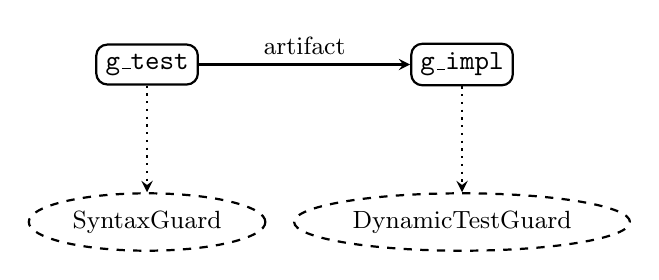
\begin{tikzpicture}[node distance=2cm, auto, >=stealth, thick]
    \node (test) [draw, rectangle, rounded corners] {\texttt{g\_test}};
    \node (impl) [draw, rectangle, rounded corners, right of=test, node distance=4cm] {\texttt{g\_impl}};

    \draw[->] (test) -- node[above] {\small artifact} (impl);

    \node (guard1) [draw, dashed, ellipse, below of=test] {\small SyntaxGuard};
    \node (guard2) [draw, dashed, ellipse, below of=impl] {\small DynamicTestGuard};

    \draw[->, dotted] (test) -- (guard1);
    \draw[->, dotted] (impl) -- (guard2);
\end{tikzpicture}
\end{center}

\subsection{Step 1: Test Generation (g\_test)}

\textbf{Prompt:}
\begin{lstlisting}[language=python, caption={Test Generation Prompt}]
Write pytest test functions for a Stack class
with push, pop, peek, is_empty, and size methods.
Output ONLY the test code.
\end{lstlisting}

\textbf{Generation Attempt 1:}
\begin{lstlisting}[language=python, caption={Generated Tests}]
def test_push_pop():
    s = Stack()
    s.push(1)
    assert s.pop() == 1

def test_is_empty():
    s = Stack()
    assert s.is_empty()
    s.push(1)
    assert not s.is_empty()
\end{lstlisting}

\textbf{Guard (SyntaxGuard):} $\top$ (AST parses successfully)

\textbf{State Transition:} \texttt{g\_test} $\rightarrow$ \texttt{VALIDATED}

\subsection{Step 2: Implementation Generation (g\_impl)}

\textbf{Prompt} (with artifact injection):
\begin{lstlisting}[language=python, caption={Implementation Prompt}]
Write a Python Stack class...
You must implement code that passes:
{test_code}  # <- Injected from g_test
\end{lstlisting}

\textbf{Generation Attempt 1:}
\begin{lstlisting}[language=python, caption={First Draft Implementation}]
class Stack:
    def __init__(self):
        self._items = []

    def push(self, item):
        self._items.append(item)

    def pop(self):
        return self._items.pop()  # Bug: no empty check
\end{lstlisting}

\textbf{Guard (DynamicTestGuard):} $\bot$
\begin{tcolorbox}[colback=red!5!white,colframe=red!75!black,title=Guard Feedback]
\texttt{IndexError: pop from empty list}
\end{tcolorbox}

\textbf{Context Refinement:}
\begin{lstlisting}[language={}, caption={Refinement Prompt}]
Previous attempt failed:
IndexError: pop from empty list
Fix the implementation.
\end{lstlisting}

\textbf{Generation Attempt 2:}
\begin{lstlisting}[language=python, caption={Corrected Implementation}]
class Stack:
    def __init__(self):
        self._items = []

    def push(self, item):
        self._items.append(item)

    def pop(self):
        if not self._items:
            raise IndexError("pop from empty stack")
        return self._items.pop()

    # ... (other methods omitted for brevity)
\end{lstlisting}

\textbf{Guard (DynamicTestGuard):} $\top$ (all tests pass)

\textbf{State Transition:} \texttt{g\_impl} $\rightarrow$ \texttt{VALIDATED}

\subsection{Execution Summary}

\begin{table}[h]
\centering
\begin{tabular}{@{}l c c c@{}}
\toprule
\textbf{Step} & \textbf{Attempts} & \textbf{Guard Result} & \textbf{Duration} \\
\midrule
g\_test & 1 & $\top$ & 2.3s \\
g\_impl & 2 & $\top$ & 4.1s \\
\bottomrule
\end{tabular}
\end{table}

\noindent \textbf{Total retries:} 1 \\
\textbf{Total duration:} 6.4s \\
\textbf{Workflow state:} \texttt{COMPLETE}

\section{Bootstrapping Legacy Systems}
\label{appendix:legacy}

The framework as presented assumes workflows begin with explicit specifications. Legacy (``brownfield'') systems present a practical challenge: the specification exists only implicitly in running code. There are no tests to validate against, no documented invariants to enforce.

This appendix sketches how the framework might be extended to support bootstrapping---generating the missing validation infrastructure from existing codebases. The approach is not novel; it formalizes characterization testing practices that predate this work \cite{feathers2004working}.

\subsection{The Initialization Problem}

In greenfield systems, guards have well-defined pass/fail semantics from the start. In brownfield systems, we face a chicken-and-egg problem: we cannot validate code without tests, but we cannot write tests without understanding the code's actual behavior.

Formally, for a legacy artifact $a_{legacy}$ and guard $G_i$, the initial state is undefined---we lack the predicate to evaluate. The bootstrapping problem is to construct that predicate by observing the system's behavior.

\subsection{Characterization Testing as Guard Generation}

The standard TDD relationship (code must satisfy tests) reverses during bootstrapping: tests must satisfy code. The legacy system becomes the oracle.

\begin{center}
\begin{tabular}{@{}l l l@{}}
\toprule
\textbf{Approach} & \textbf{Oracle} & \textbf{Artifact Under Test} \\
\midrule
Standard TDD & Tests & Code must satisfy tests \\
Bootstrapping & Code & Tests must satisfy code \\
\bottomrule
\end{tabular}
\end{center}

This has a practical consequence: test failure during bootstrapping indicates a bug in the \textit{test}, not the system under test. The guard accepts tests only when they pass against unmodified legacy code---including behavior that might be considered bugs in a greenfield context but are now load-bearing ``features.''

\subsection{A Three-Phase Pipeline}

The bootstrapping process can be decomposed into three phases. These are not novel contributions---they reflect standard practice in legacy system modernization---but expressing them as guard predicates allows integration with the framework.

\subsubsection{Phase I: Structural Audit}

The first phase establishes what can be analyzed without execution.

\begin{guardbox}{\textbf{G$_{24}$}: LEGACY $\rightarrow$ ANALYZED}
$
\begin{aligned}
& \pred{ast\_parseable}(a) \\
& \land \pred{imports\_resolvable}(a) \\
& \land \pred{no\_syntax\_errors}(a)
\end{aligned}
$
\end{guardbox}

\begin{guardbox}{\textbf{G$_{25}$}: ANALYZED $\rightarrow$ DEPENDENCY\_MAPPED}
$
\begin{aligned}
& \pred{call\_graph\_extracted}(a) \\
& \land \pred{module\_boundaries\_identified}(a) \\
& \land \pred{entry\_points\_documented}(a)
\end{aligned}
$
\end{guardbox}

\noindent \textbf{Output:} Dependency graph, module boundaries, entry points---the structural map needed for targeted characterization.

\subsubsection{Phase II: Characterization Testing}

Characterization tests capture what the system \emph{does}, not what it \emph{should} do. The legacy code is the oracle.

\begin{guardbox}{\textbf{G$_{26}$}: DEPENDENCY\_MAPPED $\rightarrow$ CHARACTERIZED}
$
\begin{aligned}
& \pred{generated\_tests\_pass}(a, a_{legacy}) \\
& \land \pred{covers\_observed\_behavior}(a) \\
& \land \pred{edge\_cases\_captured}(a)
\end{aligned}
$
\end{guardbox}

\begin{guardbox}{\textbf{G$_{27}$}: CHARACTERIZED $\rightarrow$ COVERAGE\_SUFFICIENT}
$
\begin{aligned}
& \pred{line\_coverage}(a) \geq \theta_{line} \\
& \land \pred{branch\_coverage}(a) \geq \theta_{branch} \\
& \land \pred{critical\_paths\_covered}(a)
\end{aligned}
$
\end{guardbox}

\begin{remark}[Untestable Code]
Code that resists characterization testing often indicates dead code, error handlers for impossible conditions, or race conditions. These require manual analysis via HumanGuard (G$_{20}$) rather than automated characterization.
\end{remark}

\subsubsection{Phase III: Constraint Promotion}

Characterization tests become constraints. The system transitions from ``undefined state'' to ``guarded state.''

\begin{guardbox}{\textbf{G$_{28}$}: COVERAGE\_SUFFICIENT $\rightarrow$ GAPS\_IDENTIFIED}
$
\begin{aligned}
& \pred{untested\_paths\_flagged}(a) \\
& \land \pred{mutation\_survivors\_logged}(a) \\
& \land \pred{risk\_assessment\_complete}(a)
\end{aligned}
$
\end{guardbox}

\begin{guardbox}{\textbf{G$_{29}$}: CHARACTERIZED $\rightarrow$ REFACTOR\_SAFE}
$
\begin{aligned}
& \pred{behavior\_preserved}(a', a_{legacy}) \\
& \land \pred{tests\_still\_pass}(a') \\
& \land \pred{no\_new\_warnings}(a')
\end{aligned}
$
\end{guardbox}

\noindent Once G$_{29}$ passes, the legacy system has bootstrapped into a standard guarded workflow---future changes must satisfy the characterization tests. The system transitions from ``we don't know what this code does'' to ``we have tests that document what it does, and changes must preserve that behavior.''

This is not a guarantee of correctness in any absolute sense. The characterization tests capture observed behavior, which may include bugs. The value is that \textit{changes} are now guarded---regressions become detectable.

\subsection{Bootstrap Workflow DAG}

\begin{center}
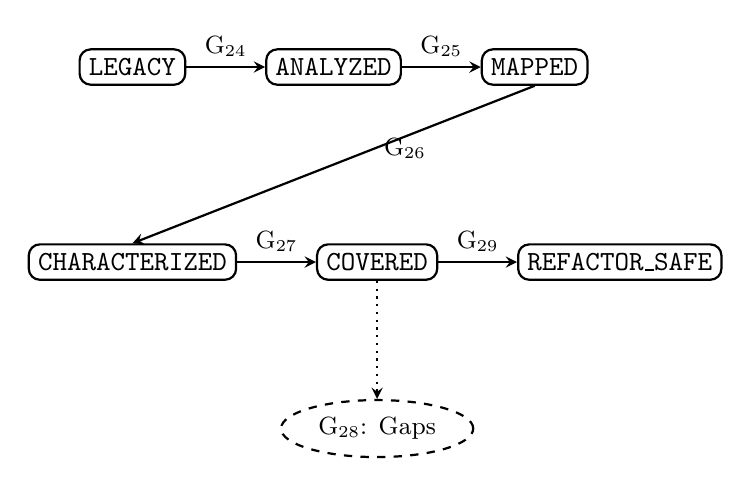
\begin{tikzpicture}[
    % 1. Increase node distance and define separate vertical/horizontal spacing
    node distance=1.5cm and 1.0cm,
    auto,
    >=stealth,
    thick,
    % 2. Define a style for your boxes to keep code clean
    block/.style={rectangle, draw, rounded corners, align=center}
]

    % --- ROW 1 ---
    \node (legacy) [block] {\texttt{LEGACY}};
    % Use 'right=of' (requires \usetikzlibrary{positioning}) to avoid overlap
    \node (analyzed) [block, right=of legacy] {\texttt{ANALYZED}};
    \node (mapped) [block, right=of analyzed] {\texttt{MAPPED}};

    % --- ROW 2 ---
    % Position 'char' below 'legacy' to start the second row
    \node (char) [block, below=of legacy, yshift=-0.5cm] {\texttt{CHARACTERIZED}};
    \node (covered) [block, right=of char] {\texttt{COVERED}};
    \node (safe) [block, right=of covered] {\texttt{REFACTOR\_SAFE}};

    % --- EDGES ROW 1 ---
    \draw[->] (legacy) -- node[above] {\small G$_{24}$} (analyzed);
    \draw[->] (analyzed) -- node[above] {\small G$_{25}$} (mapped);

    % --- TRANSITION EDGE (Diagonal) ---
    % Drawing from Mapped South to Char North or East looks cleaner
    \draw[->] (mapped.south) -- node[right, pos=0.4] {\small G$_{26}$} (char.north);

    % --- EDGES ROW 2 ---
    \draw[->] (char) -- node[above] {\small G$_{27}$} (covered);
    \draw[->] (covered) -- node[above] {\small G$_{29}$} (safe);

    % --- GAPS NODE ---
    \node (gaps) [draw, dashed, ellipse, below=of covered] {\small G$_{28}$: Gaps};
    \draw[->, dotted] (covered) -- (gaps);

\end{tikzpicture}
\end{center}
\end{document}
